% Options for packages loaded elsewhere
\PassOptionsToPackage{unicode}{hyperref}
\PassOptionsToPackage{hyphens}{url}
%
\documentclass[
]{article}
\usepackage{amsmath,amssymb}
\usepackage{iftex}
\ifPDFTeX
  \usepackage[T1]{fontenc}
  \usepackage[utf8]{inputenc}
  \usepackage{textcomp} % provide euro and other symbols
\else % if luatex or xetex
  \usepackage{unicode-math} % this also loads fontspec
  \defaultfontfeatures{Scale=MatchLowercase}
  \defaultfontfeatures[\rmfamily]{Ligatures=TeX,Scale=1}
\fi
\usepackage{lmodern}
\ifPDFTeX\else
  % xetex/luatex font selection
\fi
% Use upquote if available, for straight quotes in verbatim environments
\IfFileExists{upquote.sty}{\usepackage{upquote}}{}
\IfFileExists{microtype.sty}{% use microtype if available
  \usepackage[]{microtype}
  \UseMicrotypeSet[protrusion]{basicmath} % disable protrusion for tt fonts
}{}
\makeatletter
\@ifundefined{KOMAClassName}{% if non-KOMA class
  \IfFileExists{parskip.sty}{%
    \usepackage{parskip}
  }{% else
    \setlength{\parindent}{0pt}
    \setlength{\parskip}{6pt plus 2pt minus 1pt}}
}{% if KOMA class
  \KOMAoptions{parskip=half}}
\makeatother
\usepackage{xcolor}
\usepackage[left=1.5in, right=1.5in, top=1in, bottom=1in]{geometry}
\usepackage{longtable,booktabs,array}
\usepackage{calc} % for calculating minipage widths
% Correct order of tables after \paragraph or \subparagraph
\usepackage{etoolbox}
\makeatletter
\patchcmd\longtable{\par}{\if@noskipsec\mbox{}\fi\par}{}{}
\makeatother
% Allow footnotes in longtable head/foot
\IfFileExists{footnotehyper.sty}{\usepackage{footnotehyper}}{\usepackage{footnote}}
\makesavenoteenv{longtable}
\usepackage{graphicx}
\makeatletter
\newsavebox\pandoc@box
\newcommand*\pandocbounded[1]{% scales image to fit in text height/width
  \sbox\pandoc@box{#1}%
  \Gscale@div\@tempa{\textheight}{\dimexpr\ht\pandoc@box+\dp\pandoc@box\relax}%
  \Gscale@div\@tempb{\linewidth}{\wd\pandoc@box}%
  \ifdim\@tempb\p@<\@tempa\p@\let\@tempa\@tempb\fi% select the smaller of both
  \ifdim\@tempa\p@<\p@\scalebox{\@tempa}{\usebox\pandoc@box}%
  \else\usebox{\pandoc@box}%
  \fi%
}
% Set default figure placement to htbp
\def\fps@figure{htbp}
\makeatother
\setlength{\emergencystretch}{3em} % prevent overfull lines
\providecommand{\tightlist}{%
  \setlength{\itemsep}{0pt}\setlength{\parskip}{0pt}}
\setcounter{secnumdepth}{5}
\usepackage{booktabs}
\usepackage{threeparttable}
\usepackage[utf8]{inputenc}
\usepackage[T1]{fontenc}
\usepackage{amsmath}
\usepackage{tabularx}
\usepackage{threeparttable}
\usepackage{pdflscape}
\usepackage{float}
\floatplacement{figure}{H}
\usepackage{subcaption}
\usepackage{caption}
\captionsetup[figure]{skip=0.5em}
\usepackage{booktabs}
\usepackage{longtable}
\usepackage{array}
\usepackage{multirow}
\usepackage{wrapfig}
\usepackage{float}
\usepackage{colortbl}
\usepackage{pdflscape}
\usepackage{tabu}
\usepackage{threeparttable}
\usepackage{threeparttablex}
\usepackage[normalem]{ulem}
\usepackage{makecell}
\usepackage{xcolor}
\usepackage[]{natbib}
\bibliographystyle{apalike}
\usepackage{bookmark}
\IfFileExists{xurl.sty}{\usepackage{xurl}}{} % add URL line breaks if available
\urlstyle{same}
\hypersetup{
  pdftitle={Imagine -- An Exploratory Analysis v3},
  hidelinks,
  pdfcreator={LaTeX via pandoc}}

\title{Imagine -- An Exploratory Analysis v3}
\author{}
\date{\vspace{-2.5em}}

\begin{document}
\maketitle

\section{Data Merging, Filtering, and Data
Transformation}\label{data-merging-filtering-and-data-transformation}

Sense and feature annotation datasets were merged using \texttt{\$id}
and \texttt{\$no}, as suggested by Nina. Sense annotations by ARB were
ignored, since they only span 100 rows. Rows with non-numeric values in
either feature variable or a non-NA value in \texttt{\$Exclusions} (from
the sense annotation data) were removed. Of the 38 remaining cases where
NCH and AH's sense annotations disagreed, 38 were settled via majority
vote using a third coder (referee) who separately annotated exactly
these disagreement cases; the 0 cases where all three coders disagreed
have no majority and were marked unclassifiable. This leaves 906
observations. Further, rows with sense values
\texttt{"?-UNCLASSIFIABLE"}, \texttt{"5-EXCLAMATIVE"}, or
\texttt{"O-Other"} (not occurring) were dropped due to low occurrence
(see Table \ref{tab:senseCounts}), which makes estimation unstable. The
final dataset consists of 893 observations. Lastly, the three feature
dimensions were \(z\)-scaled for comparability.

\begin{table}[H]
\centering
\caption{\label{tab:unnamed-chunk-2}\label{tab:senseCounts} Sense counts before removal of edge classes.}
\centering
\begin{tabular}[t]{lr}
\toprule
Sense & N\\
\midrule
?-UNCLASSIFIABLE & 5\\
1-VIZUALIZE/PICTURE & 518\\
2-THINK/BELIVE & 224\\
3-SUPPOSE/ASSUME & 92\\
4-FALSE\_PERCEPTION & 59\\
5-EXCLAMATIVE & 8\\
\bottomrule
\end{tabular}
\end{table}

\section{Descriptive Statistics}\label{descriptive-statistics}

Figure \ref{fig:distributions} shows considerable overlap in feature
distributions across the different senses. To quantify this, we computed
pairwise overlap coefficients between sense distributions for each
feature using kernel density estimation (KDE), measuring both the raw
shared area under the minimum of two KDE curves and its normalization by
each sense's total density (see Table \ref{tab:overlap} in the
Appendix). Figure \ref{fig:Xdistributions} shows a similar picture for
feature interactions. In view of that, clear sense separation via
feature dimensions seems unlikely.

\begin{figure}[h]

{\centering 
\includegraphics[width=1\linewidth]{imagine_report_v3_files/figure-latex/unnamed-chunk-3-1} 

}

\caption{Fetaure distributions for the different senses\label{fig:distributions}}\label{fig:unnamed-chunk-3}
\end{figure}

\begin{figure}[h]

{\centering 
\includegraphics[width=1\linewidth]{imagine_report_v3_files/figure-latex/unnamed-chunk-4-1} 

}

\caption{Interactions of feature distributions for the different senses\label{fig:Xdistributions}}\label{fig:unnamed-chunk-4}
\end{figure}

\subsection{\texorpdfstring{Why is intentionality so narrowly peaked for
\texttt{"1-VIZUALIZE/PICTURE"}?}{Why is intentionality so narrowly peaked for "1-VIZUALIZE/PICTURE"?}}\label{why-is-intentionality-so-narrowly-peaked-for-1-vizualizepicture}

The intentionality panel of Figure \ref{fig:distributions} shows a
markedly narrower peak for \texttt{"1-VIZUALIZE/PICTURE"} than for the
other senses. Table \ref{tab:sdByFeature} confirms this is a localized
pattern: the standard deviation of intentionality for
\texttt{"1-VIZUALIZE/PICTURE"} is roughly a third to a quarter of the
other senses', whereas factivity and pictoriality show no comparable
narrowing for this sense.

\begin{table}[H]
\centering
\caption{\label{tab:unnamed-chunk-5}Standard deviation (raw 1--7 scale) of each feature by sense.\label{tab:sdByFeature}}
\centering
\begin{tabular}[t]{lrrr}
\toprule
Sense & Factivity & Intentionality & Pictoriality\\
\midrule
1-VIZUALIZE/PICTURE & 1.56 & 0.41 & 1.87\\
2-THINK/BELIVE & 1.41 & 1.72 & 1.13\\
3-SUPPOSE/ASSUME & 1.45 & 1.88 & 0.87\\
4-FALSE\_PERCEPTION & 1.14 & 1.57 & 1.52\\
\bottomrule
\end{tabular}
\end{table}

To check whether this is an artifact of averaging over disagreeing
coders, we used the un-aggregated per-coder scores loaded in
\texttt{import-additional-data}, which combines two coding-batch files
that together cover the full corpus:
\texttt{raw\_feature\_scores\_pt1.xlsx} (tokens no. 1--100, scored by
three coders, N, D, and E) and \texttt{raw\_feature\_scores\_pt2.xlsx}
(tokens no. 101--1000, scored by two coders, D and N, plus a precomputed
mean). Raw coder-level records were available for 893 of the 893
observations (0 missing, 0\%). Table \ref{tab:coderAgreement} compares
the D and N coders, who scored every token in both batches (the third
coder E, present only for tokens no. 1--100, is not included in this
comparison); it shows that both coders \emph{individually} already rate
\texttt{"1-VIZUALIZE/PICTURE"} tokens with low variance on
intentionality (SD \(\approx\) 0.3--0.65) and close to the scale ceiling
(mean \(\approx\) 6 out of 7), whereas their variance for the other
senses is far higher (SD \(\approx\) 1.3--2.0). Mean absolute
disagreement between coders is also the same size or smaller for
\texttt{"1-VIZUALIZE/PICTURE"} than for the other senses. In other
words, the narrow peak is not a symptom of coders disagreeing and
averaging out to a bland middle value -- each coder already converges on
a high intentionality score for this sense.

\begin{table}[H]
\centering
\caption{\label{tab:unnamed-chunk-6}Per-coder intentionality agreement by sense (raw 1--7 scale). D and N denote the two coders.\label{tab:coderAgreement}}
\centering
\begin{tabular}[t]{lrrrrrrr}
\toprule
Sense & $n$ & Mean D & Mean N & SD D & SD N & Mean $|D-N|$ & $r_{D,N}$\\
\midrule
1-VIZUALIZE/PICTURE & 518 & 6.03 & 6.05 & 0.32 & 0.68 & 0.42 & 0.22\\
2-THINK/BELIVE & 224 & 3.67 & 3.42 & 1.99 & 1.69 & 0.72 & 0.78\\
3-SUPPOSE/ASSUME & 92 & 4.45 & 4.17 & 1.98 & 1.86 & 0.42 & 0.94\\
4-FALSE\_PERCEPTION & 59 & 3.58 & 4.15 & 2.00 & 1.41 & 1.12 & 0.72\\
\bottomrule
\end{tabular}
\end{table}

The coder correlation \(r_{D,N}\) is nonetheless the weakest for
\texttt{"1-VIZUALIZE/PICTURE"} (0.22) despite the low absolute
disagreement. This is consistent with a restriction-of-range effect:
once most ratings are compressed near the top of the scale, there is
little residual variance left for the two coders' scores to correlate
over, even though they remain close in absolute terms.

Taken together, the pattern looks like a genuine ceiling effect rather
than a data or annotation artifact: \texttt{"1-VIZUALIZE/PICTURE"}
denotes deliberately forming a mental image, which by definition is an
intentional act, so both coders independently push intentionality
ratings toward the top of the scale for this sense. Factivity and
pictoriality carry no such definitional constraint and show no
equivalent narrowing.

\section{Predictive Modeling of Sense
Membership}\label{predictive-modeling-of-sense-membership}

To characterize how annotation dimensions jointly predict latent sense
membership, we fit a multinomial generalized linear model with ridge
(L2) regularization. Manual sense annotations served as the dependent
variable. Predictors included all three annotation dimensions and their
pairwise interactions. Regularization strength was selected via
cross-validation to promote coefficient stability.

The multinomial model achieved a cross-validated accuracy of 75.6\% with
optimal \(\lambda\)=0.034. Performance was highly uneven across senses,
however. Table \ref{tab:senseAccuracy} details accuracy per sense:

\begin{itemize}
\tightlist
\item
  \texttt{"1-VISUALIZE/PICTURE"} was recovered with high accuracy
  (97.1\%) and high posterior concentration
  (\(\tilde{p}_{\max}\)=0.824), indicating a well-defined feature
  region.
\item
  \texttt{"2-THINK/BELIEVE"} showed moderate accuracy (73.7\%) with
  correspondingly moderate confidence (\(\tilde{p}_{\max}\)=0.634).
\item
  \texttt{"3-SUPPOSE/ASSUME"} \& \texttt{"4-FALSE\_PERCEPTION"} were not
  reliably recovered (accuracy=0\% and 11.9\% respectively). Both were
  misclassified \texttt{"1-VISUALIZE/PICTURE"} or
  \texttt{"2-THINK/BELIEVE"} with low to moderate confidence
  (\(\tilde{p}_{\max}\)=0.676 and \(\tilde{p}_{\max}\)=0.567
  respectively).
\end{itemize}

\begin{table}[H]
\centering
\caption{\label{tab:unnamed-chunk-8}Posterior probability concentration and classification accuracy by sense. $\tilde{p}_{\max}$ denotes the median maximum predicted probability across observations; $\text{IQR}(\hat{p}_{\max})$ denotes the interquartile range of maximum predicted probabilities.\label{tab:senseAccuracy}}
\centering
\begin{tabular}[t]{lrrr}
\toprule
True Sense & $\tilde{p}_{\max}$ & $\text{IQR}(\hat{p}_{\max})$ & Accuracy\\
\midrule
1-VIZUALIZE/PICTURE & 0.824 & 0.177 & 0.971\\
2-THINK/BELIVE & 0.634 & 0.193 & 0.737\\
3-SUPPOSE/ASSUME & 0.676 & 0.180 & 0.000\\
4-FALSE\_PERCEPTION & 0.567 & 0.243 & 0.119\\
\bottomrule
\end{tabular}
\end{table}

Precision, recall, and F1 are reported in Table \ref{tab:cmDetail}. Note
that the precision and F1 for \texttt{"3-SUPPOSE/ASSUME"} is NA because
it was never correctly classified. Table \ref{tab:cm} in the Appendix
details the the confusion matrix by sense.

\begin{table}[H]
\centering
\caption{\label{tab:unnamed-chunk-9}Confusion Matrix.\label{tab:cmDetail}}
\centering
\begin{tabular}[t]{lrrr}
\toprule
  & Precision & Recall & F1\\
\midrule
Class: 1-VIZUALIZE/PICTURE & 0.7933754 & 0.9710425 & 0.8732639\\
Class: 2-THINK/BELIVE & 0.6653226 & 0.7366071 & 0.6991525\\
Class: 3-SUPPOSE/ASSUME &  & 0.0000000 & \\
Class: 4-FALSE\_PERCEPTION & 0.6363636 & 0.1186441 & 0.2000000\\
\bottomrule
\end{tabular}
\end{table}

These results indicate that the three features define a robust two-way
opposition between \texttt{"1-VISUALIZE/PICTURE"} and
\texttt{"2-THINK/BELIEVE"}, but are insufficient to distinguish the
remaining senses.

As a robustness check, we assessed coefficient stability using
nonparametric bootstrapping (500 resamples). Bootstrap confidence
intervals were narrow across main effects and interactions (Figure
\ref{fig:bootstrapping}), indicating that the fitted probability
surfaces were numerically stable under resampling. Keep in mind that
estimates for \texttt{"3-SUPPOSE/ASSUME"} and
\texttt{"FALSE\_PERCEPTION"} should be interpreted cautiously.

\begin{figure}[h]

{\centering 
\includegraphics[width=1\linewidth]{imagine_report_v3_files/figure-latex/unnamed-chunk-10-1} 

}

\caption{Bootstrapped Coefficients (n = 500) with 95\% CI.\label{fig:bootstrapping}}\label{fig:unnamed-chunk-10}
\end{figure}

Predicted probabilities based on the optimal model were generated across
the observed range of each pair of annotation dimensions while holding
the third dimension constant at its median. These predictions were
visualized in Figure \ref{fig:Xeffects} as two-dimensional heatmaps to
facilitate interpretation of interaction patterns.

\begin{figure}[h]

{\centering 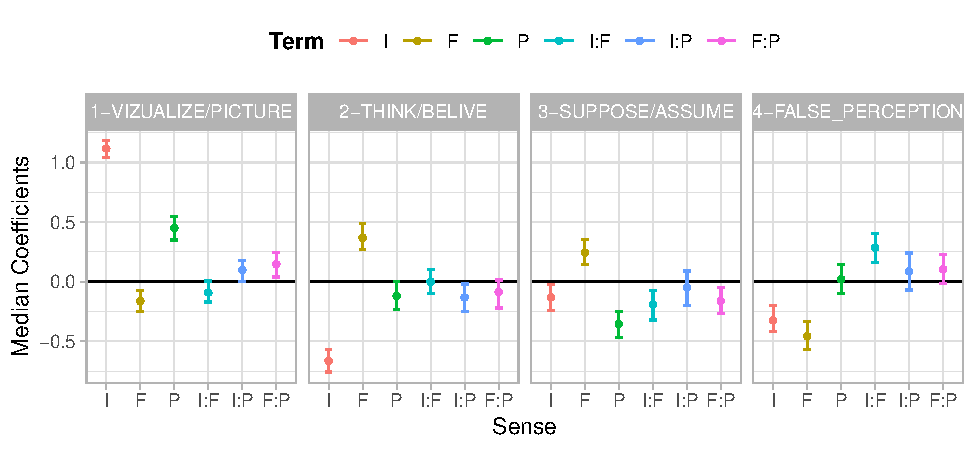
\includegraphics[width=1\linewidth]{imagine_report_v3_files/figure-latex/unnamed-chunk-11-1} 

}

\caption{redicted sense probability based on GLM with ridge regularization for 2-way interactions. The third dimension is held constant at the median value.\label{fig:Xeffects}}\label{fig:unnamed-chunk-11}
\end{figure}

\subsection{Robustness check: hierarchical (nested)
classification}\label{robustness-check-hierarchical-nested-classification}

Given how uneven performance is across senses (Table
\ref{tab:senseAccuracy}), we checked whether a hierarchical
decomposition -- first separating \texttt{"1-VIZUALIZE/PICTURE"} from
the rest, then \texttt{"2-THINK/BELIVE"} from the remainder, and finally
\texttt{"3-SUPPOSE/ASSUME"} from \texttt{"4-FALSE\_PERCEPTION"} -- could
better exploit whatever local structure exists among the
harder-to-classify senses. Each split was fit as a ridge (L2)
regularized logistic regression on the same three annotation dimensions
and their pairwise interactions, with \(\lambda\) again selected via
cross-validation. This is a robustness check on the modeling strategy,
not a replacement for the multinomial model reported above.

Table \ref{tab:nodeAccuracy} shows that, evaluated in isolation on only
the observations relevant to it, each split separates reasonably well --
including the \texttt{"3-SUPPOSE/ASSUME"}
vs.~\texttt{"4-FALSE\_PERCEPTION"} split, which reaches 83.4\% accuracy
on its own.

\begin{table}[H]
\centering
\caption{\label{tab:unnamed-chunk-13}Node-local accuracy of each split in the hierarchical cascade, evaluated on the subset of observations relevant to that split.\label{tab:nodeAccuracy}}
\centering
\begin{tabular}[t]{lrr}
\toprule
Split & $n$ & Accuracy\\
\midrule
A: 1-VIZUALIZE/PICTURE vs. rest & 893 & 0.839\\
B: 2-THINK/BELIVE vs. rest (within non-1) & 375 & 0.691\\
C: 3-SUPPOSE/ASSUME vs. 4-FALSE\_PERCEPTION & 151 & 0.834\\
\bottomrule
\end{tabular}
\end{table}

Chaining the splits into a single cascade -- as the model would actually
be used -- tells a different story, however. Overall accuracy is 74.7\%,
effectively unchanged from the flat multinomial model's 75.6\% (Table
\ref{tab:hierAccuracy}). \texttt{"3-SUPPOSE/ASSUME"} is still never
recovered (0\% recall), and \texttt{"4-FALSE\_PERCEPTION"} improves only
modestly (25.4\% recall, up from 11.9\% in the flat model).

\begin{table}[H]
\centering
\caption{\label{tab:unnamed-chunk-14}Hierarchical model: precision, recall, and F1 by sense.\label{tab:hierAccuracy}}
\centering
\begin{tabular}[t]{lrrr}
\toprule
  & Precision & Recall & F1\\
\midrule
Class: 1-VIZUALIZE/PICTURE & 0.8213058 & 0.9227799 & 0.8690909\\
Class: 2-THINK/BELIVE & 0.6062718 & 0.7767857 & 0.6810176\\
Class: 3-SUPPOSE/ASSUME & 0.0000000 & 0.0000000 & \\
Class: 4-FALSE\_PERCEPTION & 0.6521739 & 0.2542373 & 0.3658537\\
\bottomrule
\end{tabular}
\end{table}

The discrepancy between the node-local and cascaded results is explained
by where \texttt{"3-SUPPOSE/ASSUME"} observations actually end up:
nearly all of them are already claimed by node A or node B before ever
reaching node C, where the 3-vs-4 split would otherwise do reasonably
well. The node C split is locally accurate but almost never reached by
genuine \texttt{"3-SUPPOSE/ASSUME"} tokens in practice, because they are
indistinguishable from \texttt{"1-VIZUALIZE/PICTURE"} and
\texttt{"2-THINK/BELIVE"} earlier in the cascade. This is consistent
with the pairwise KDE overlap analysis (Table \ref{tab:overlap}) and the
distributions in Figure \ref{fig:distributions}, which already showed no
distinct feature-space region for \texttt{"3-SUPPOSE/ASSUME"}: the
bottleneck is a lack of separating signal in the three annotation
dimensions themselves, not the flat multinomial model's shared
parameterization. Hierarchical decomposition therefore does not resolve
the poor recoverability of \texttt{"3-SUPPOSE/ASSUME"} and
\texttt{"4-FALSE\_PERCEPTION"}.

\subsection{Robustness check: coder-reliability weighted
models}\label{robustness-check-coder-reliability-weighted-models}

The three annotation dimensions are themselves aggregates over multiple
coders, and the coder-agreement analysis above (Table
\ref{tab:coderAgreement}) showed that agreement varies considerably by
sense and dimension. We checked whether accounting for this --
downweighting rows and dimensions where coders disagreed more -- changes
the model's ability to recover \texttt{"3-SUPPOSE/ASSUME"} and
\texttt{"4-FALSE\_PERCEPTION"}. For each observation and each dimension
we computed the standard deviation across that row's available raw coder
scores (three coders, N/D/E, for tokens no. 1--100; two coders, D/N, for
tokens no. 101--1000 -- SD is well-defined for either count, so no
special-casing is needed). Reliability was then defined as
\(w = 1 / (1 + \text{SD})\), so perfectly agreeing coders yield \(w=1\)
and reliability decays as disagreement grows. Because \texttt{glmnet}
only accepts a single weight per observation, not one per feature per
observation, we tried three different ways of injecting this row- and
dimension-specific reliability into the same ridge multinomial model
used above, none of which replace it.

The 0, 1, and 23 rows with fewer than two usable raw scores for
intentionality, factivity, and pictoriality respectively were imputed
with that dimension's corpus median SD, a neutral ``typical
reliability'' placeholder, before computing the weights below.

\textbf{Variant 1 -- attenuate the feature values.} For each row and
dimension we multiply the \(z\)-scored value by that row's own
reliability weight for that dimension \emph{before} forming the main
effects and interactions, so noisier per-row measurements are shrunk
toward zero and contribute less to the fit -- preserving the row- and
dimension-specific granularity, at the cost of changing the actual
feature values the model sees rather than just their loss weight.

\textbf{Variant 2 -- a single per-row weight.} We collapse the three
dimension-specific reliabilities into one weight per row (their average)
and pass it to \texttt{glmnet}'s native \texttt{weights} argument,
leaving the feature values themselves untouched. This is the more
standard ``weighted regression'' reading, at the cost of no longer
distinguishing a row that is reliable on one dimension but noisy on
another.

\textbf{Variant 3 -- a corpus-wide penalty per dimension.} Instead of a
row-level adjustment, we compute one reliability score per dimension
across the whole corpus (its mean SD) and translate that into
\texttt{glmnet}`s \texttt{penalty.factor}, so that a systematically
noisier dimension is shrunk more by the ridge penalty; an interaction
term's penalty is the product of its two parent dimensions' penalties.
This ignores row-to-row variation entirely, but is the reading closest
to ``weight the feature dimensions'' taken literally.

Table \ref{tab:weightedComparison} compares overall accuracy and
per-sense recall across the unweighted model and all three weighted
variants.

\begin{table}[H]
\centering
\caption{\label{tab:unnamed-chunk-19}Overall accuracy and per-sense recall: unweighted model vs. three coder-reliability weighted variants. Recall 1--4 refer to \texttt{1-VIZUALIZE/PICTURE}, \texttt{2-THINK/BELIVE}, \texttt{3-SUPPOSE/ASSUME}, and \texttt{4-FALSE\_PERCEPTION} respectively.\label{tab:weightedComparison}}
\centering
\fontsize{9}{11}\selectfont
\begin{tabular}[t]{lrrrrr}
\toprule
Model & Acc. & Recall 1 & Recall 2 & Recall 3 & Recall 4\\
\midrule
Baseline (unweighted) & 0.756 & 0.971 & 0.737 & 0 & 0.119\\
V1: attenuated features & 0.741 & 0.983 & 0.661 & 0 & 0.085\\
V2: per-row weight & 0.749 & 0.977 & 0.710 & 0 & 0.068\\
V3: per-dim. penalty & 0.750 & 0.979 & 0.710 & 0 & 0.068\\
\bottomrule
\end{tabular}
\end{table}

None of the three weighting schemes improve recovery of
\texttt{"3-SUPPOSE/ASSUME"} (recall stays at 0 in all three variants,
same as the unweighted model) or \texttt{"4-FALSE\_PERCEPTION"} (recall
is flat or slightly worse than the unweighted model's 11.9\%). Overall
accuracy is essentially unchanged or marginally lower across all three
variants. This is a second, independent robustness check pointing to the
same conclusion as the hierarchical model above: the difficulty in
recovering \texttt{"3-SUPPOSE/ASSUME"} and
\texttt{"4-FALSE\_PERCEPTION"} is not an artifact of noisy per-row
annotation that reliability weighting could correct for -- it reflects a
genuine lack of separating signal between these senses and
\texttt{"1-VIZUALIZE/PICTURE"}/\texttt{"2-THINK/BELIVE"} in the three
annotation dimensions themselves.

\subsection{Robustness check: interaction order and a nonparametric
ceiling}\label{robustness-check-interaction-order-and-a-nonparametric-ceiling}

The model above assumes a specific functional form: main effects plus
all pairwise interactions between the three annotation dimensions. We
checked whether that assumption, rather than the dimensions themselves,
is limiting recovery of \texttt{"3-SUPPOSE/ASSUME"} and
\texttt{"4-FALSE\_PERCEPTION"}, in two ways. First, since there are only
three predictors, extending the ridge model to include the full
three-way interaction costs a single extra column and is essentially
free to try. Second, and more informatively, we fit a fully
nonparametric random forest on the same three raw features with no
manually specified interaction terms at all, as an upper bound on what
\emph{any} function of these three features -- linear, polynomial, or
otherwise -- could achieve.

Table \ref{tab:interactionComparison} compares the baseline two-way
model, the three-way interaction, and the random forest (both in-sample
and OOB) on overall accuracy and per-sense recall.

\begin{table}[H]
\centering
\caption{\label{tab:unnamed-chunk-22}Overall accuracy and per-sense recall: baseline two-way model vs. three-way interaction and random forest. Recall 1--4 refer to \texttt{1-VIZUALIZE/PICTURE}, \texttt{2-THINK/BELIVE}, \texttt{3-SUPPOSE/ASSUME}, and \texttt{4-FALSE\_PERCEPTION} respectively.\label{tab:interactionComparison}}
\centering
\fontsize{9}{11}\selectfont
\begin{tabular}[t]{lrrrrr}
\toprule
Model & Acc. & Recall 1 & Recall 2 & Recall 3 & Recall 4\\
\midrule
Baseline (2-way) & 0.756 & 0.971 & 0.737 & 0.000 & 0.119\\
3-way interaction & 0.757 & 0.971 & 0.737 & 0.000 & 0.136\\
Random forest (in-sample) & 0.807 & 0.967 & 0.795 & 0.196 & 0.407\\
Random forest (OOB) & 0.747 & 0.940 & 0.719 & 0.043 & 0.254\\
\bottomrule
\end{tabular}
\end{table}

The three-way interaction changes almost nothing (75.6\% \(\to\) 75.7\%
accuracy; \texttt{"3-SUPPOSE/ASSUME"} recall stays at 0), so interaction
order beyond pairwise terms is not the bottleneck. The random forest
tells a more mixed story. Its in-sample accuracy (80.7\%) is inflated by
overfitting -- unsurprising given how flexible the model is relative to
the sample size, especially for the smaller senses -- but the honest,
OOB accuracy (74.7\%) is close to the baseline overall. Sense-by-sense,
though, OOB recall for \texttt{"4-FALSE\_PERCEPTION"} rises to 25.4\%,
roughly double the baseline's 11.9\%, while \texttt{"3-SUPPOSE/ASSUME"}
remains essentially unrecoverable at 4.3\% even under a fully flexible
model. This suggests the linear/fixed-interaction-order assumption of
the ridge multinomial genuinely was somewhat limiting for
\texttt{"4-FALSE\_PERCEPTION"} specifically -- a nonlinear or
non-additive combination of the three dimensions carries some real, if
modest, signal for that sense -- whereas \texttt{"3-SUPPOSE/ASSUME"}
still shows no recoverable signal even when the model is allowed to be
maximally flexible, reinforcing the conclusion from the two robustness
checks above for that sense specifically.

\section{Embedding analysis}\label{embedding-analysis}

In addition to the statistical analysis, we leveraged contextual
embeddings of sentences containing the term \textit{imagine} to
investigate how different senses of the word are represented in latent
semantic space. This embedding analysis explores the geometric structure
of the representations, the relationship between semantic similarity and
sense membership, and the alignment of embeddings with the annotated
semantic dimensions. The approach provides a comprehensive view of how
contextual usage patterns are captured by the language model (BERT) and
how they relate to theoretical distinctions between senses.

\subsection{Sense overlap based on centroid
distance}\label{sense-overlap-based-on-centroid-distance}

For each sense, we computed the cosine distance of every
\textit{imagine} token embedding to its own sense centroid and to the
other sense centroids. We then estimated the kernel density (KDE)
distributions of these distances and calculated the overlap between the
densities. The resulting overlap scores quantify how well each sense
cluster is discriminated from the others in centroid space. Importantly,
this metric measures discriminability from cluster centers, not the
actual geometric overlap of the clusters themselves. It essentially
answers the question: ``If I pick a token at random from Sense 1, how
often could it be mistaken for Sense 2 based on centroid proximity?''
This approach does not account for the internal distribution of
embeddings within a cluster. Two clusters could substantially overlap in
the embedding space, yet the distance-to-centroid measure might still
suggest low overlap if tokens happen to be near their respective
centroids.

Figure \ref{fig:KDEdistanceCentroid_ownVSother} shows the cosine
distance of tokens for each sense to their own sense-centroid and the
other sense-centroids. The overlap fractions are detailed in Figure
\ref{fig:centroidOverlapHeatmap}.

\begin{figure}
    \centering
    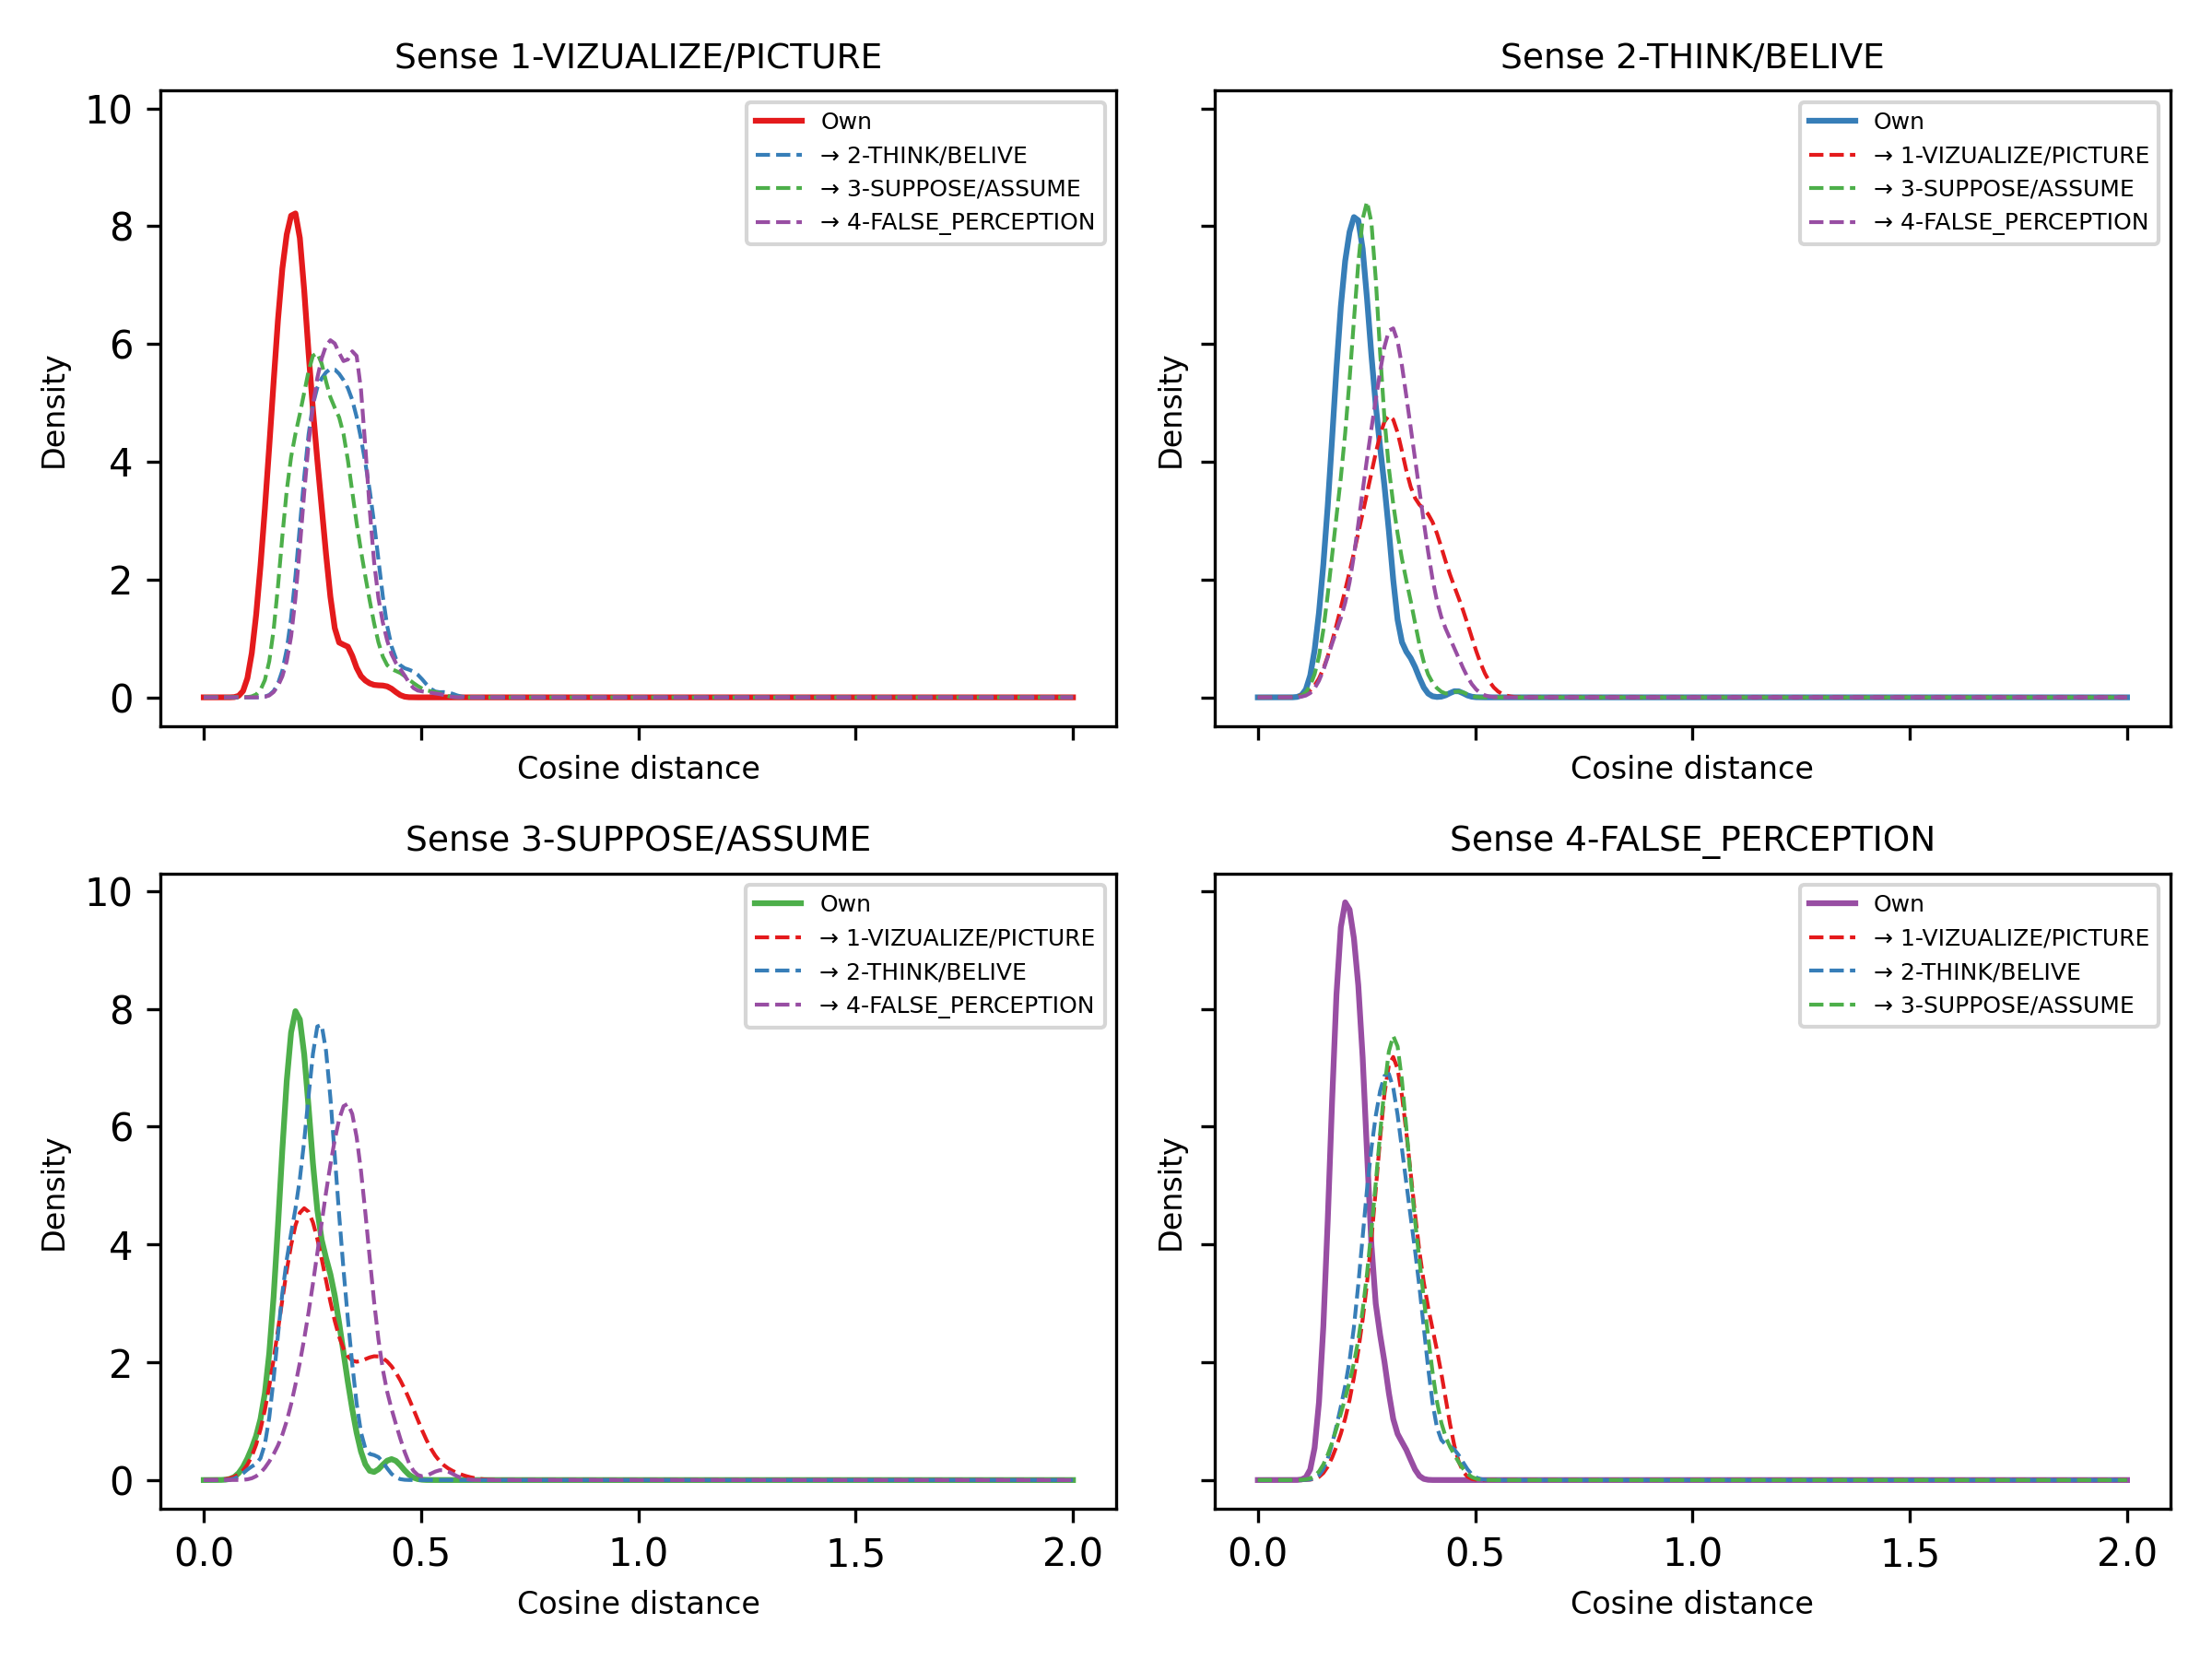
\includegraphics[width=0.8\linewidth]{../../output/plots/overlap_density_v3.png}
    \caption{Centroid-based overlap.}
    \label{fig:KDEdistanceCentroid_ownVSother}
\end{figure}

\begin{figure}[h]

{\centering 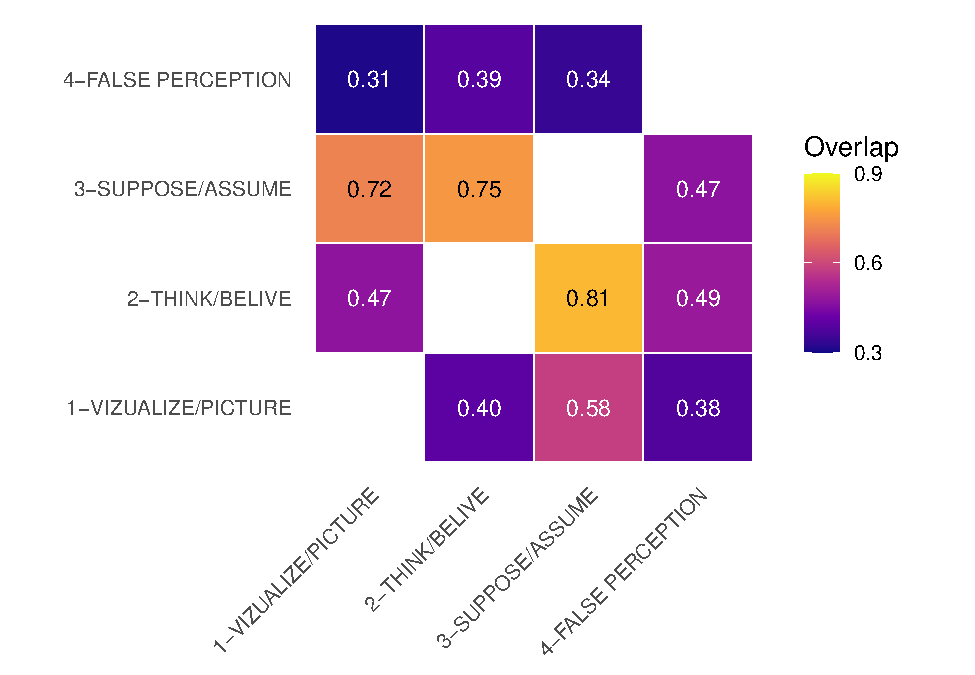
\includegraphics[width=0.6\linewidth]{imagine_report_v3_files/figure-latex/unnamed-chunk-23-1} 

}

\caption{Centroid-based overlap fractions.\label{fig:centroidOverlapHeatmap}}\label{fig:unnamed-chunk-23}
\end{figure}

\subsection{Geometric overlap}\label{geometric-overlap}

To complement the centroid-based distances, we also computed overlap
directly on the embedding distributions for each sense. For this, we
estimated KDE functions over the embeddings themselves (after 1D and 2D
PCA reduction). This yields how much of the geometric ``surface'' of one
cluster is occupied by the other. Unlike the centroid-based overlap,
which measures discriminability relative to cluster centers, this method
captures actual geometric overlap in embedding space. High overlap here
indicates that embeddings of the two senses physically occupy the same
regions, reflecting semantic entanglement or ambiguity. Low overlap
indicates that the clusters are well-separated in latent space,
regardless of centroid proximity. Thus, this analysis provides a more
direct estimate of semantic distinctiveness at the token level, whereas
centroid distances summarize separability from the average cluster
location. The overlap in 1D and 2D space is shown in Figure
\ref{fig:KDEsurface}. Figure \ref{fig:kde1dHeatmap} \&
\ref{fig:kde2dHeatmap} detail the overlap fractions, for 1D and 2D
respectively.

\begin{figure}
\centering
    \caption{Geometric overlap of different senses in embedding space.}
    \label{fig:KDEsurface}
    \begin{subfigure}[b]{0.6\textwidth}
    \centering
    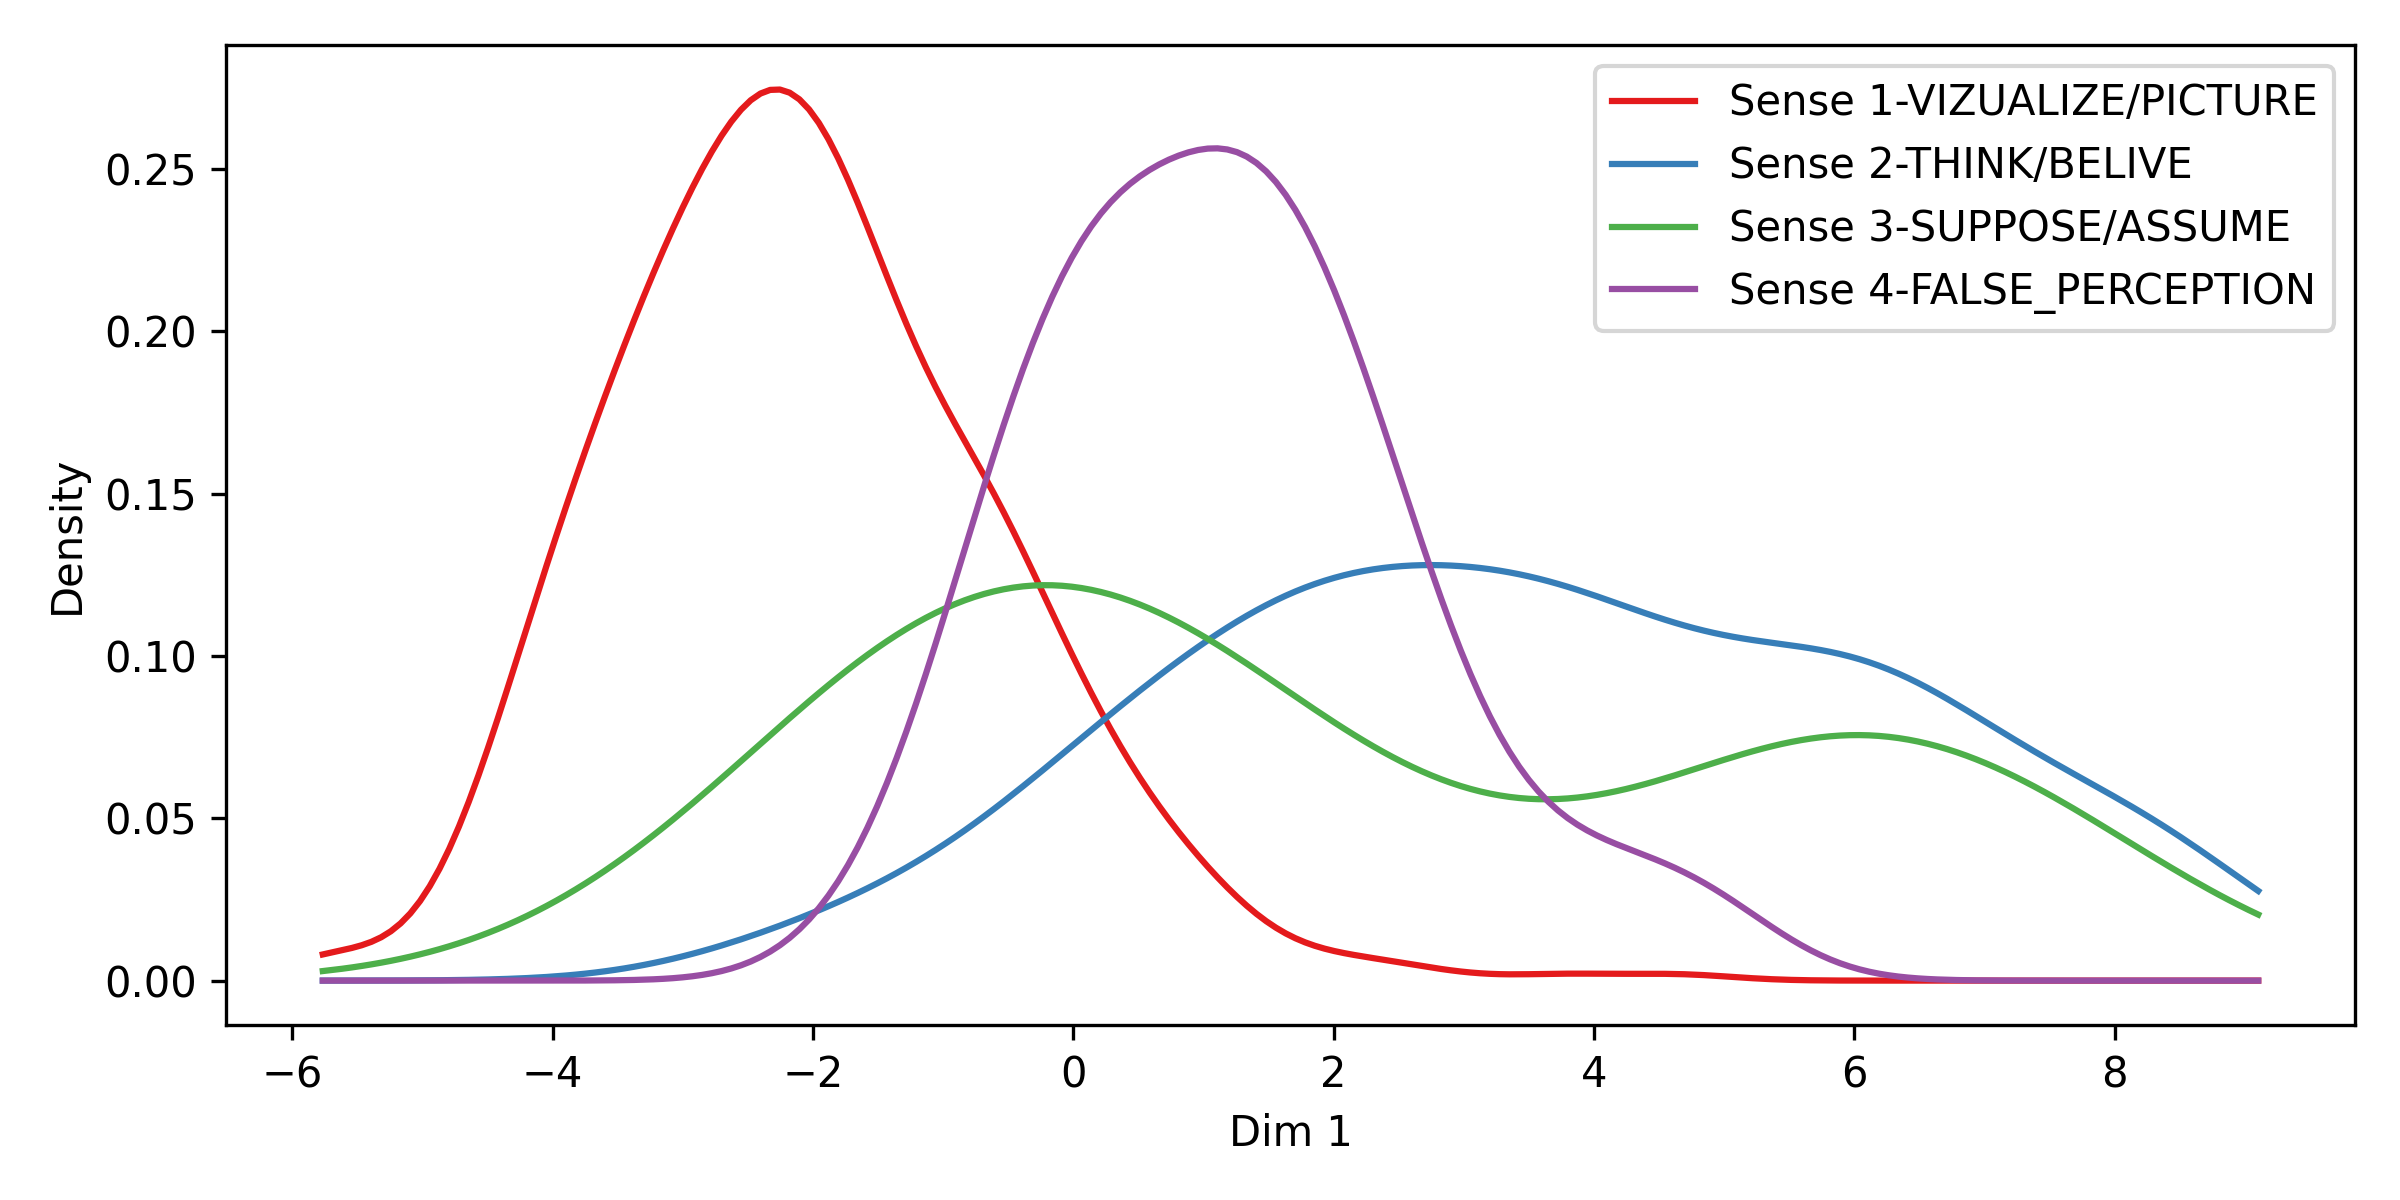
\includegraphics[width=\textwidth]{../../output/plots/kde1D_embeddings_overlap_v3.png}
    \caption{\label{fig:KDEsurface1D}}
    \end{subfigure}
    \hfill
    \begin{subfigure}[b]{0.38\textwidth}
    \centering
    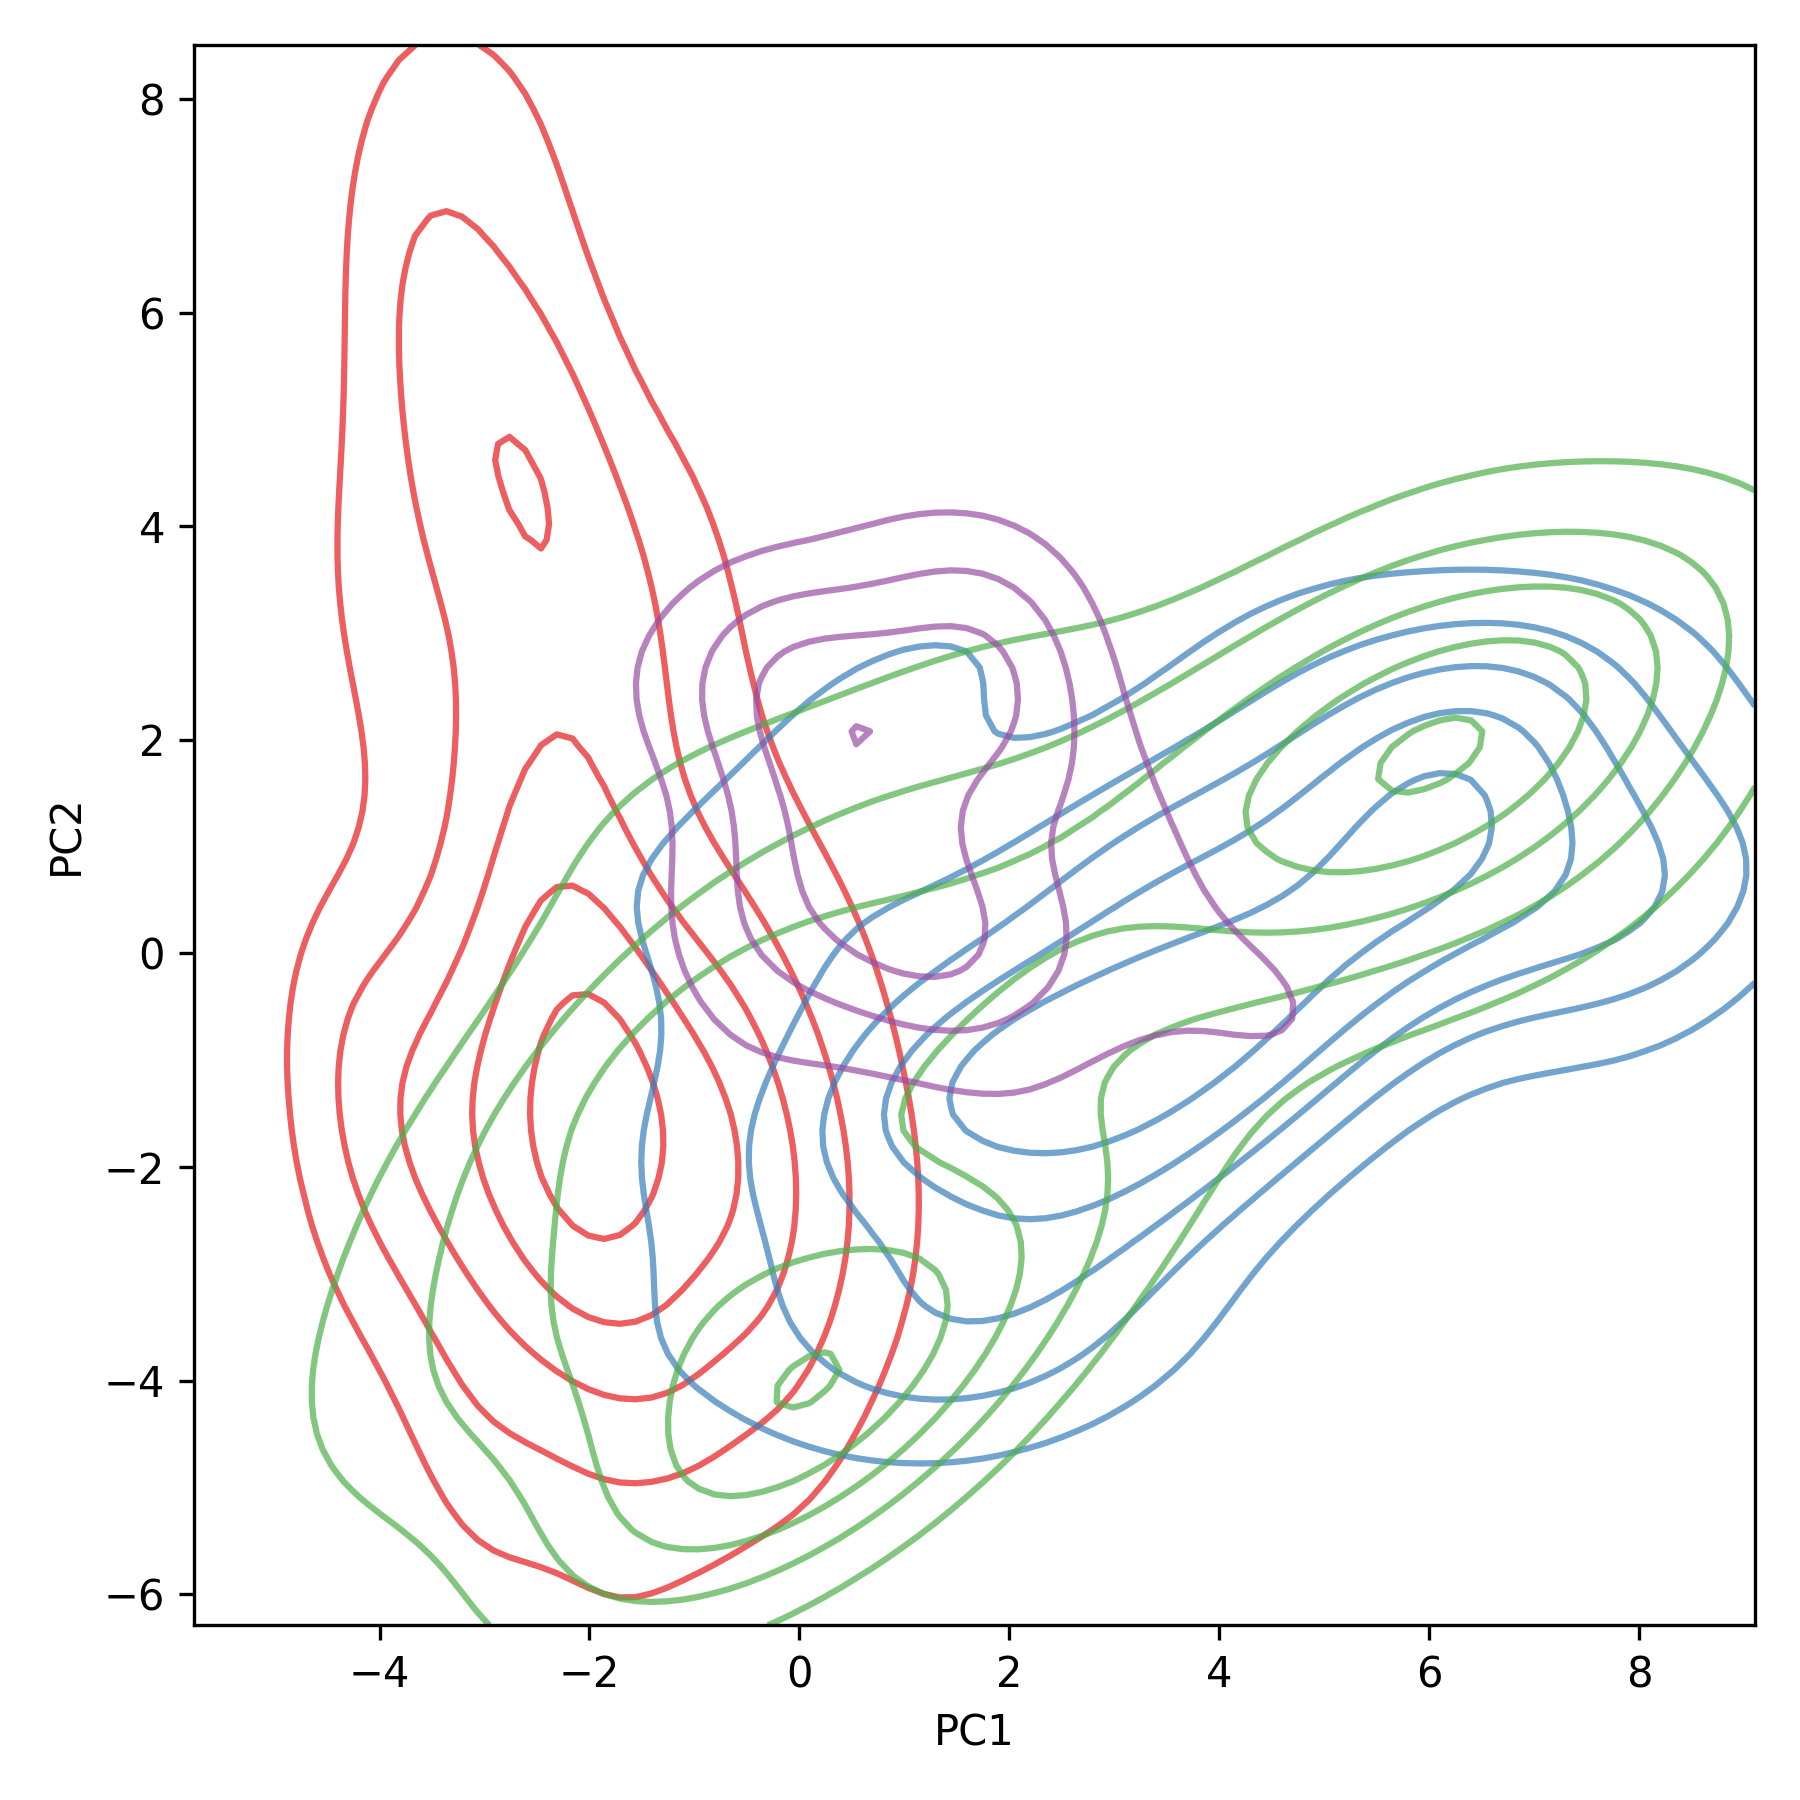
\includegraphics[width=0.9\textwidth]{../../output/plots/kde2D_embeddings_overlap_v3.png}
    \caption{\label{fig:KDEsurface1D}}
    \end{subfigure}
\end{figure}

\begin{figure}[h]

{\centering 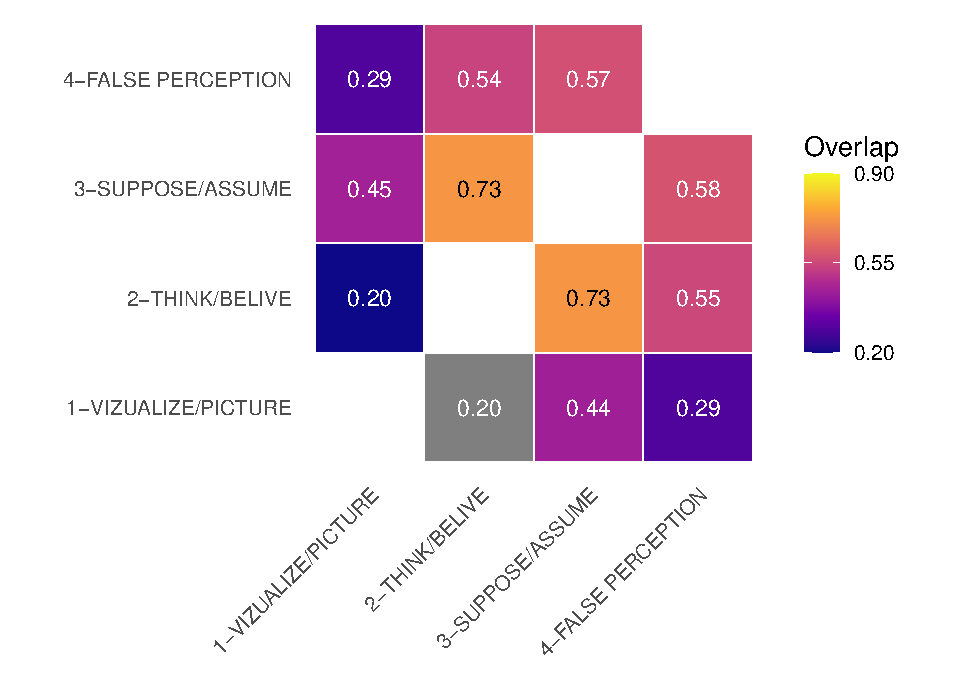
\includegraphics[width=0.6\linewidth]{imagine_report_v3_files/figure-latex/unnamed-chunk-24-1} 

}

\caption{1D KDE overlap fractions.\label{fig:kde1dHeatmap}}\label{fig:unnamed-chunk-24}
\end{figure}

\begin{figure}[h]

{\centering 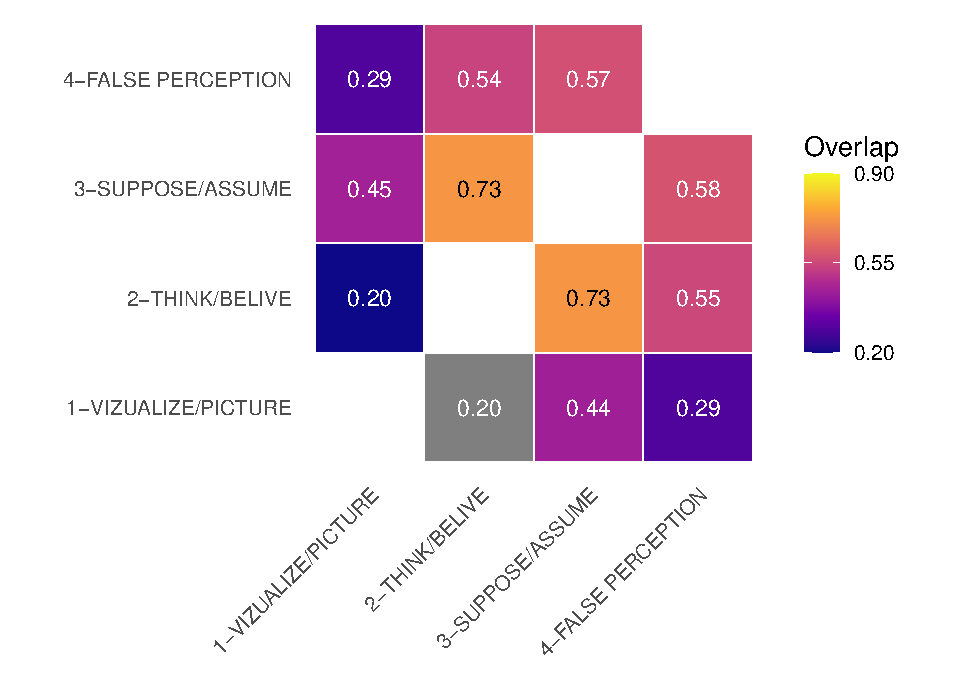
\includegraphics[width=0.6\linewidth]{imagine_report_v3_files/figure-latex/unnamed-chunk-25-1} 

}

\caption{2D KDE overlap fractions.\label{fig:kde2dHeatmap}}\label{fig:unnamed-chunk-25}
\end{figure}

\subsection{Embedding similarity vs sense
similarity}\label{embedding-similarity-vs-sense-similarity}

To examine whether sentence embeddings capture sense membership, we
computed pairwise cosine similarities between all sentence embeddings.
For comparison, a binary matrix indicated whether each sentence pair
belonged to the same annotated sense (1) or different senses (0). We
then correlated the upper-triangle values of the embedding similarity
matrix with the corresponding sense similarity values using Spearman's
rank correlation. Visualization of the results was achieved by plotting
KDE of embedding similarities for sentence pairs with the same sense
versus different senses. Higher cosine similarity for same-sense pairs
relative to different-sense pairs indicates that embeddings encode
semantic sense information. The Spearman correlation quantifies the
degree to which semantic closeness in embedding space aligns with sense
membership, providing a global measure of clustering in the latent
space. Unlike centroid-based or geometric overlap, this is a global,
distribution-agnostic summary statistic: it does not explicitly consider
clusters or shapes, only relative similarity between pairs of sentences.

Figure \ref{fig:matrixComparison} shows the distribution of pairwise
cosine similarities between sentence embeddings, separated by whether
the sentences share the same sense (red) or have different senses
(blue). Embeddings of sentences with the same sense tend to be more
similar, as evidenced by the right-shifted red distribution relative to
the blue distribution. This pattern is quantified by a Spearman
correlation of \(\rho = 0.36\) (p \textless{} 0.001), indicating a
moderate positive association between embedding similarity and sense
membership.

\begin{figure}
    \centering
    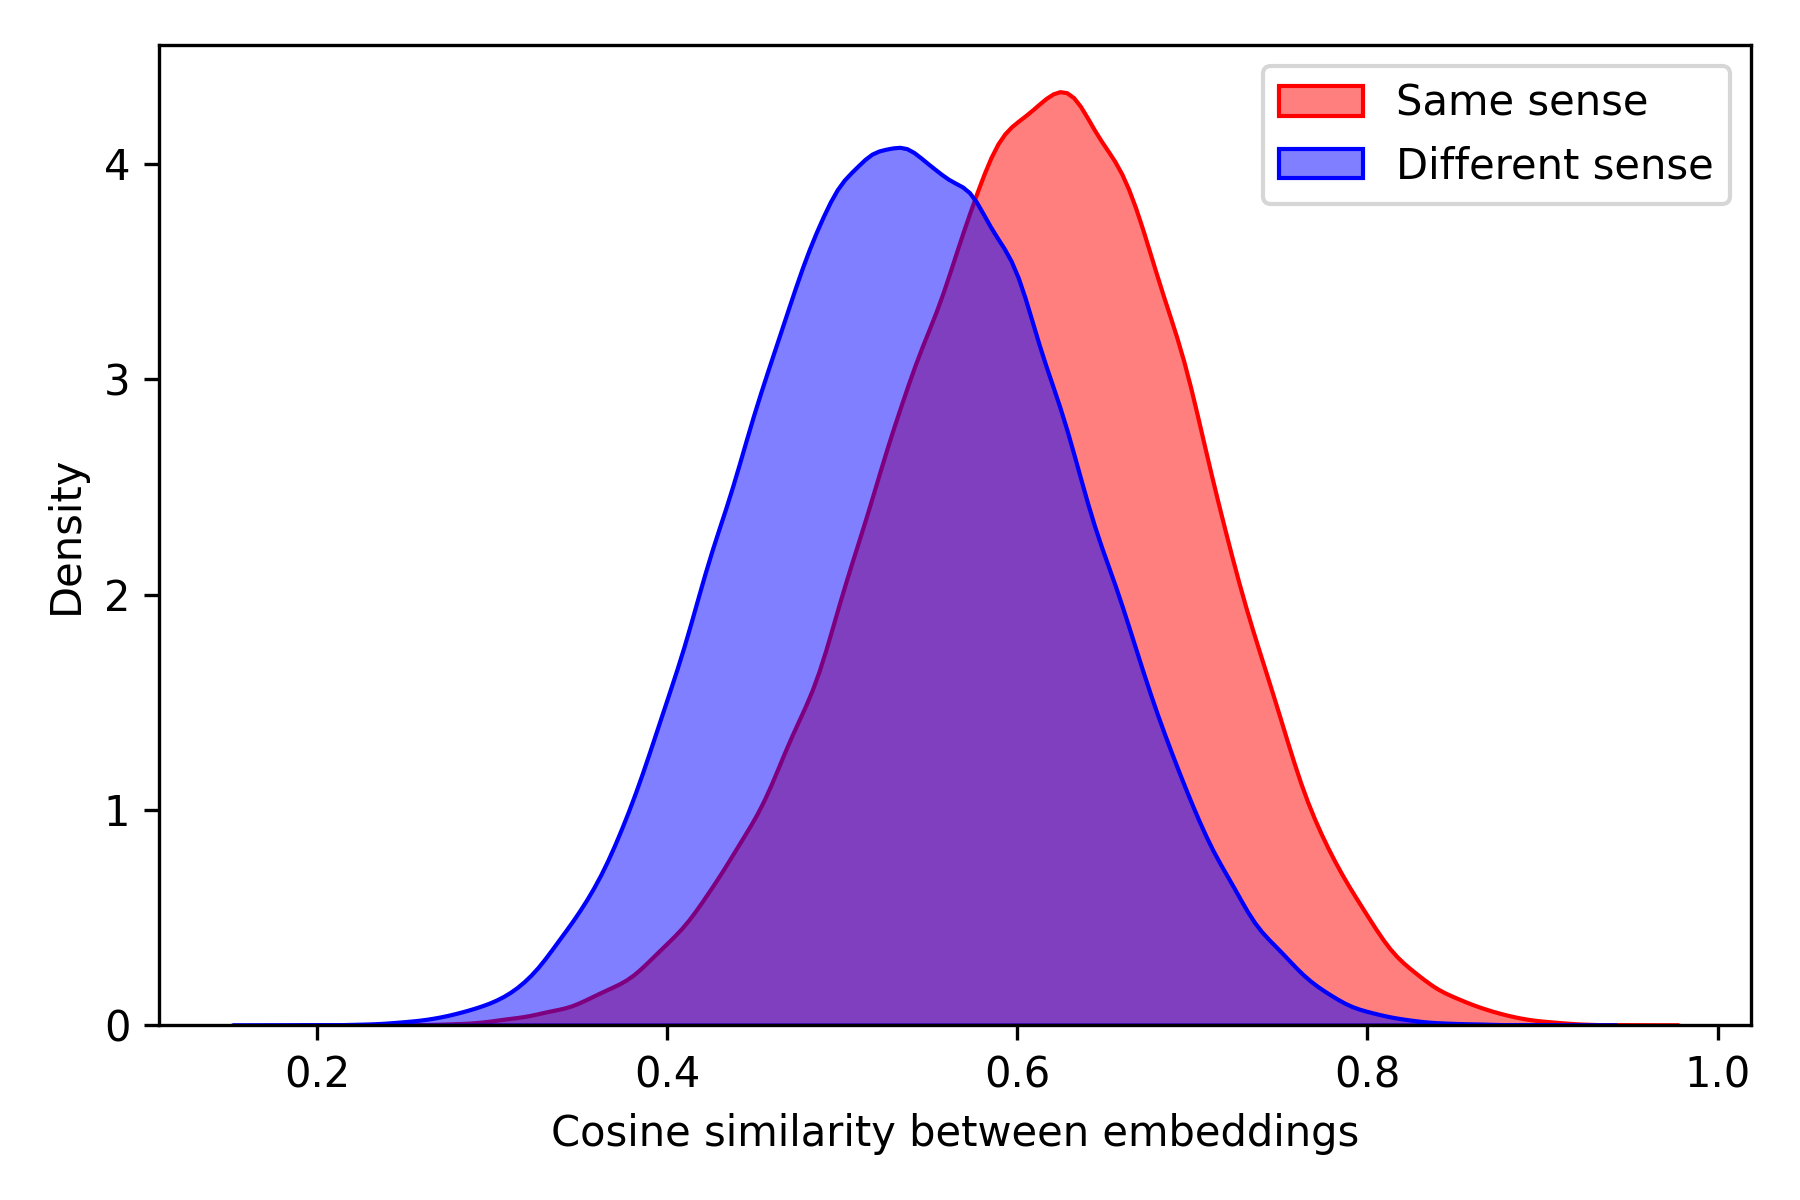
\includegraphics[width=0.5\linewidth]{../../output/plots/embedding_vs_sense_similarity_v3.png}
    \caption{Cosine similarity between same-sense and other-sense tokens of \textit{imagine}.}
    \label{fig:matrixComparison}
\end{figure}

\subsection{Senses under embedding
projection}\label{senses-under-embedding-projection}

To examine how sentence embeddings capture the annotated senses along
the three feature dimensions, we trained ridge-regularized regression
models predicting each z-scaled dimension from the sentence embeddings.
The regression coefficients define a direction in embedding space along
which the dimension increases. By projecting each sentence embedding
onto these directions, we obtain an embedding-based estimate for that
dimension. This procedure was repeated for all three dimensions,
resulting in a 3D projection of each sentence in the space spanned by
the semantic dimensions.

Here is a more detailed rundown of the analysis: Let
\(\mathbf{X} \in \mathbb{R}^{n \times d}\) denote the matrix of sentence
embeddings, where \(n\) is the number of sentences and \(d = 768\) the
embedding dimension. Let \(\mathbf{y}^{(k)} \in \mathbb{R}^n\) be the
vector of z-scaled ratings for semantic dimension
\(k \in \{\text{intentionality, factivity, pictoriality}\}\).

We fit a ridge-regularized regression model for each dimension:

\[
\hat{\boldsymbol{\beta}}^{(k)} = \operatorname*{arg\,min}_{\boldsymbol{\beta}} \left\lVert \mathbf{y}^{(k)} - \mathbf{X}\boldsymbol{\beta} \right\rVert_2^2 + \alpha \left\lVert \boldsymbol{\beta} \right\rVert_2^2,
\]

where \(\alpha \geq 0\) is a penalty strength selected via
cross-validation. Because \(d = 768\) is close to \(n\) (the number of
annotated tokens), an unregularized fit would essentially memorize the
training data without generalizing; the ridge penalty shrinks
\(\hat{\boldsymbol{\beta}}^{(k)}\) toward a more stable, generalizable
direction, the same regularization strategy used throughout the rest of
this report's models. The estimated coefficients
\(\hat{\boldsymbol{\beta}}^{(k)} \in \mathbb{R}^d\) define a direction
in embedding space corresponding to increases in dimension \(k\).

The projection of each sentence embedding \(\mathbf{x}_i\) onto this
direction provides an embedding-based estimate of the semantic
dimension:

\[
\hat{y}^{(k)}_i = \mathbf{x}_i^\top \hat{\boldsymbol{\beta}}^{(k)}, \quad i = 1, \dots, n.
\]

By computing these projections for all three dimensions, each sentence
is represented in a 3D space spanned by the semantic directions,
allowing visualization and analysis of how embeddings capture the
annotated semantic structure.

\begin{table}[H]
\centering
\caption{\label{tab:unnamed-chunk-27}Ridge regression fit predicting each feature dimension from sentence embeddings: in-sample and 5-fold cross-validated $R^2$.\label{tab:projectionR2}}
\centering
\begin{tabular}[t]{lrrrr}
\toprule
Dimension & $\alpha$ & In-sample $R^2$ & 5-fold CV $R^2$ & CV SD\\
\midrule
Intentionality & 100 & 0.840 & 0.728 & 0.039\\
Factivity & 100 & 0.640 & 0.437 & 0.056\\
Pictoriality & 100 & 0.697 & 0.495 & 0.082\\
\bottomrule
\end{tabular}
\end{table}

Table \ref{tab:projectionR2} shows that the in-sample \(R^2\) is
optimistic relative to the honest, cross-validated estimate, as expected
-- but the cross-validated \(R^2\) itself is far from zero: 0.73 for
intentionality, 0.5 for pictoriality, and 0.44 for factivity. The
embeddings therefore do carry substantial, generalizable information
about these dimensions -- particularly intentionality -- contrary to
what a purely visual read of the projection space might suggest.

Figure \ref{fig:3Dprojection} shows the 3D projection of sentence
embeddings onto the directions corresponding to the feature dimensions.
\texttt{"1-VIZUALIZE/PICTURE"} (red) separates fairly clearly from the
other three senses along the intentionality axis, consistent with both
the cross-validated \(R^2\) above and the intentionality ceiling effect
for this sense documented in Figure \ref{fig:distributions}.
\texttt{"2-THINK/BELIVE"}, \texttt{"3-SUPPOSE/ASSUME"}, and
\texttt{"4-FALSE\_PERCEPTION"}, however, remain thoroughly intermixed
with each other in this space. This is not a sign that the embeddings
fail to encode the feature dimensions -- the \(R^2\) values above show
they do -- but rather that, once the dimensions are reconstructed from
the embeddings, \texttt{"2-THINK/BELIVE"}, \texttt{"3-SUPPOSE/ASSUME"},
and \texttt{"4-FALSE\_PERCEPTION"} occupy overlapping regions of that
space, mirroring the same pattern documented throughout this report
(Figure \ref{fig:distributions}, Table \ref{tab:overlap}, and the
predictive modeling robustness checks): \texttt{"1-VIZUALIZE/PICTURE"}
is comparatively well-defined, while the other three senses are not
cleanly separated by these three dimensions, however they are estimated.

\begin{figure}
    \centering
    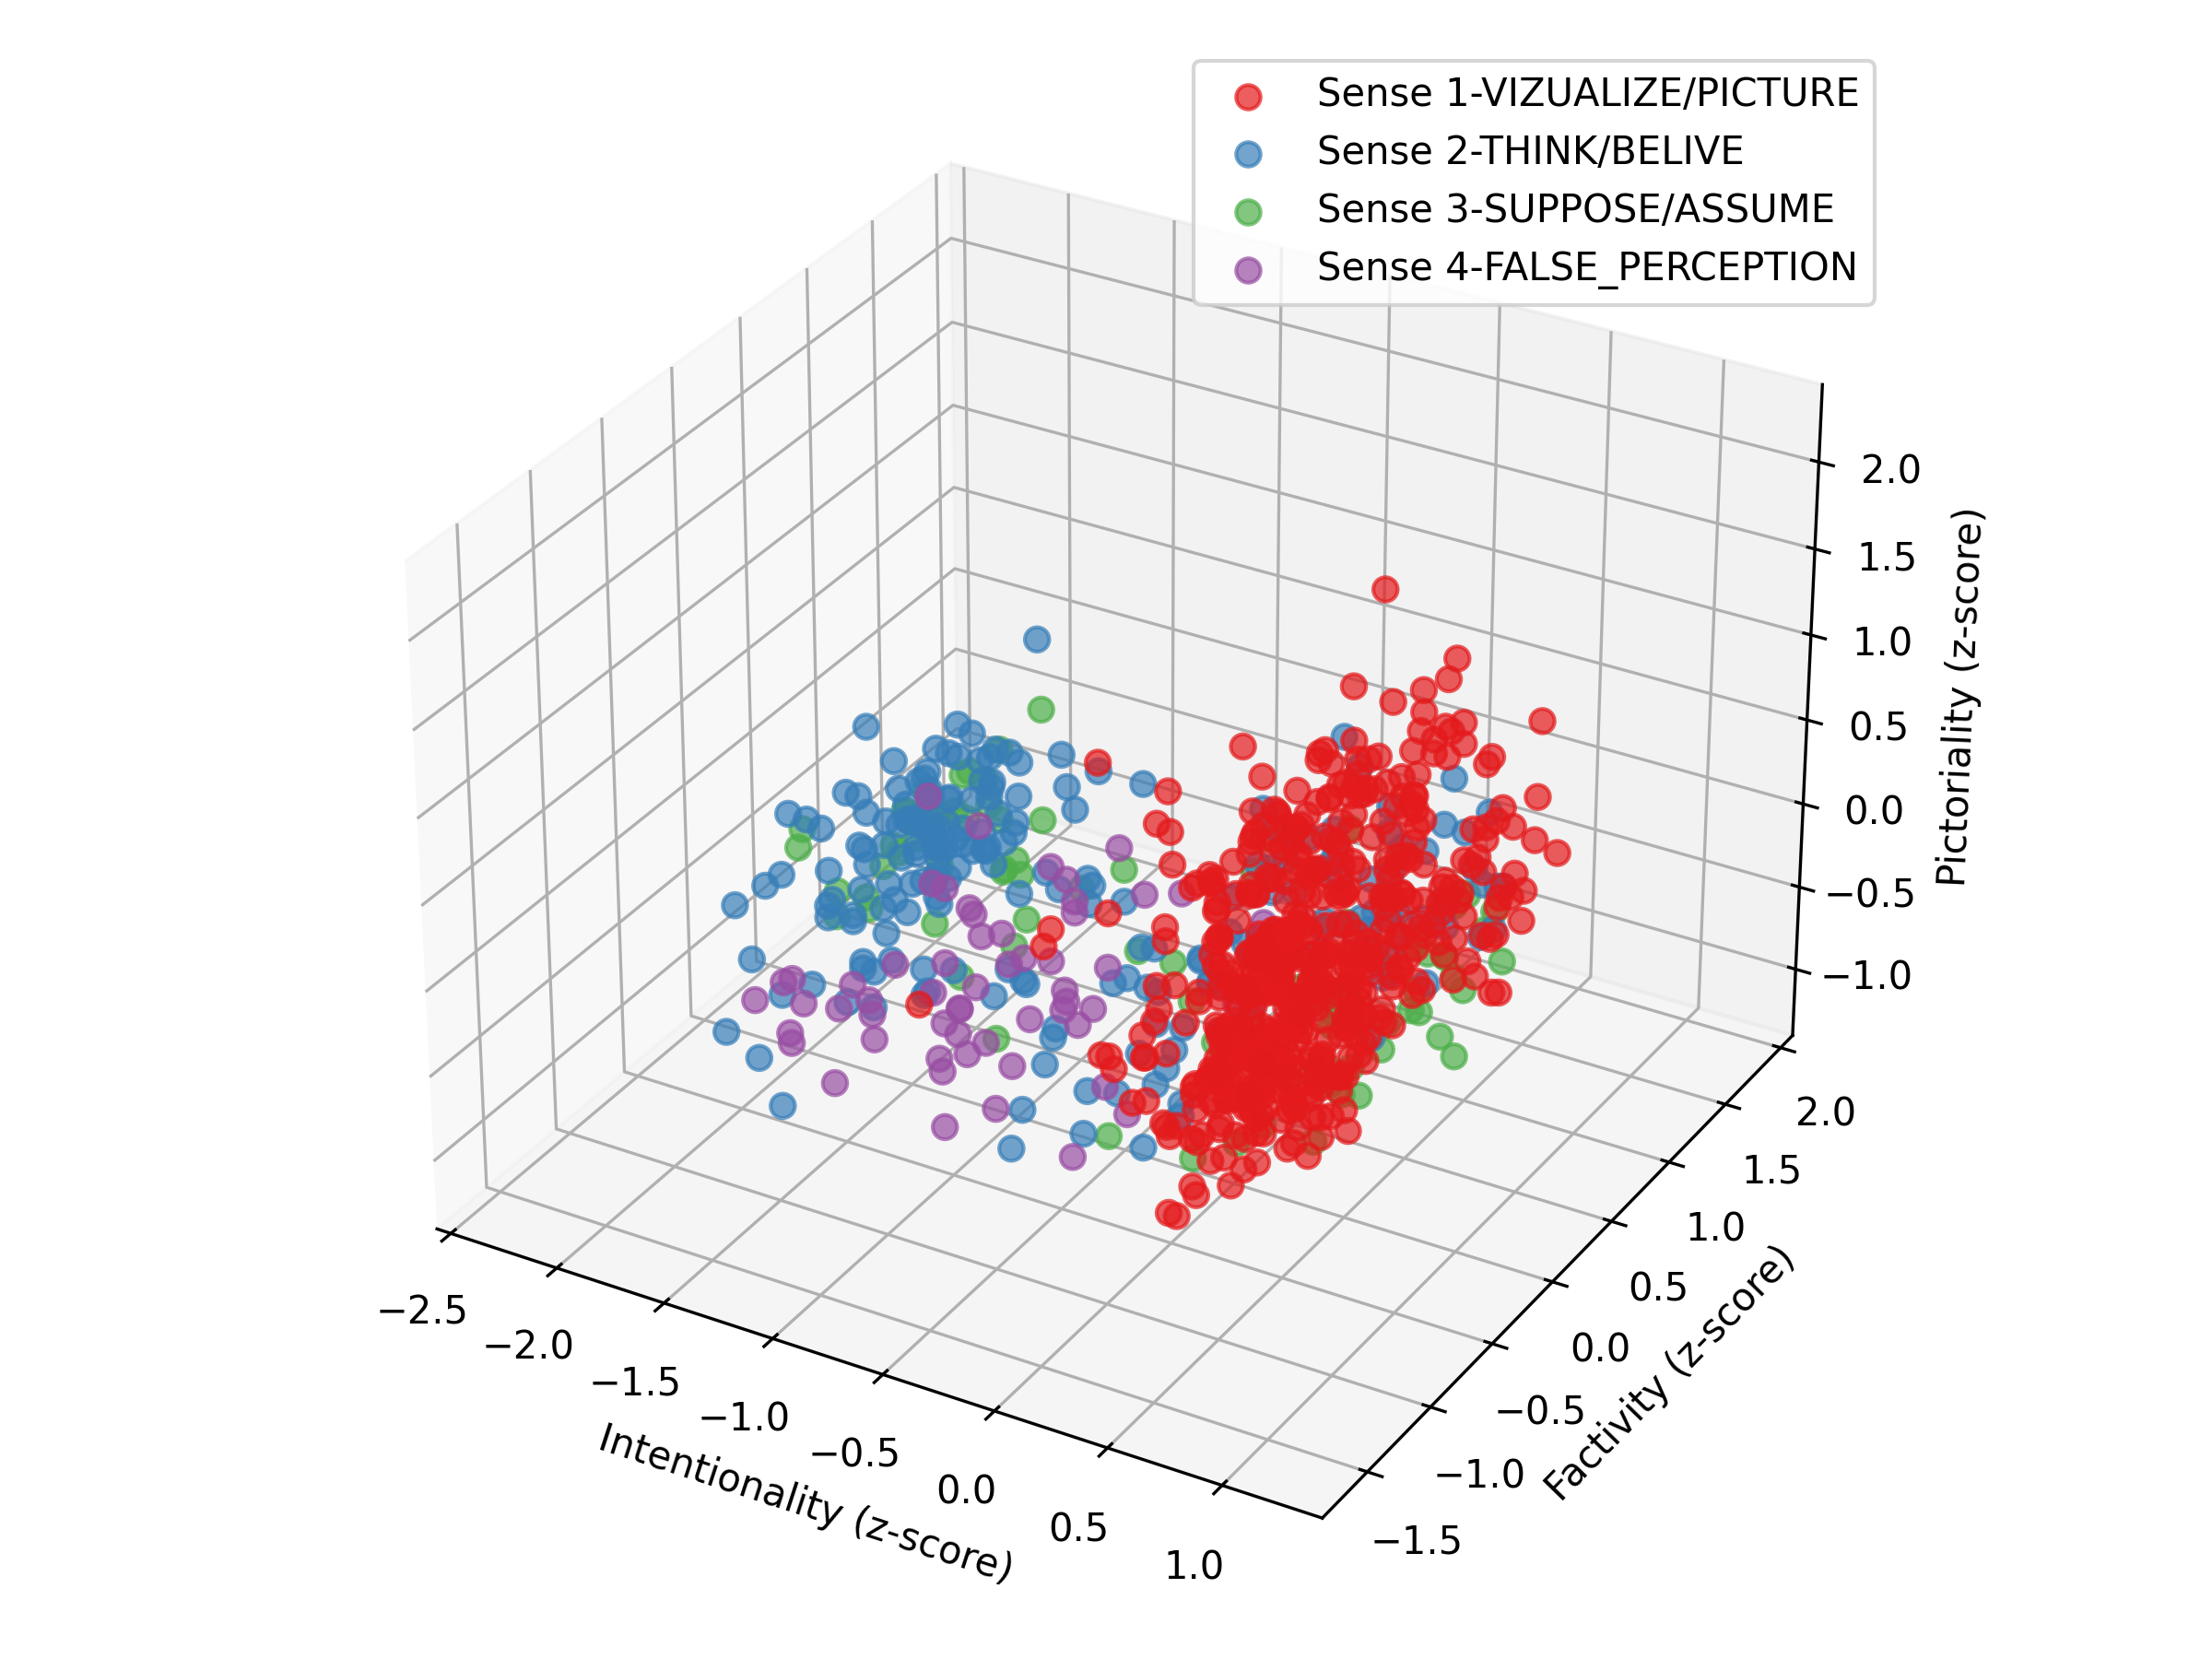
\includegraphics[width=0.5\linewidth]{../../output/plots/embedding_projection_3D_v3.png}
    \caption{3D embedding projections.}
    \label{fig:3Dprojection}
\end{figure}

Figure \ref{fig:2Dprojection} depicts 2-dimensional KDE plots for all
combinations of dimensions. \texttt{"1-VIZUALIZE/PICTURE"} again stands
out as a distinct high-density region (most visibly against
pictoriality), while the other three senses' contours overlap heavily
throughout.

\begin{figure}
\centering
    \caption{2D embedding projections.}
    \label{fig:2Dprojection}
    \begin{subfigure}[b]{0.30\textwidth}
    \centering
    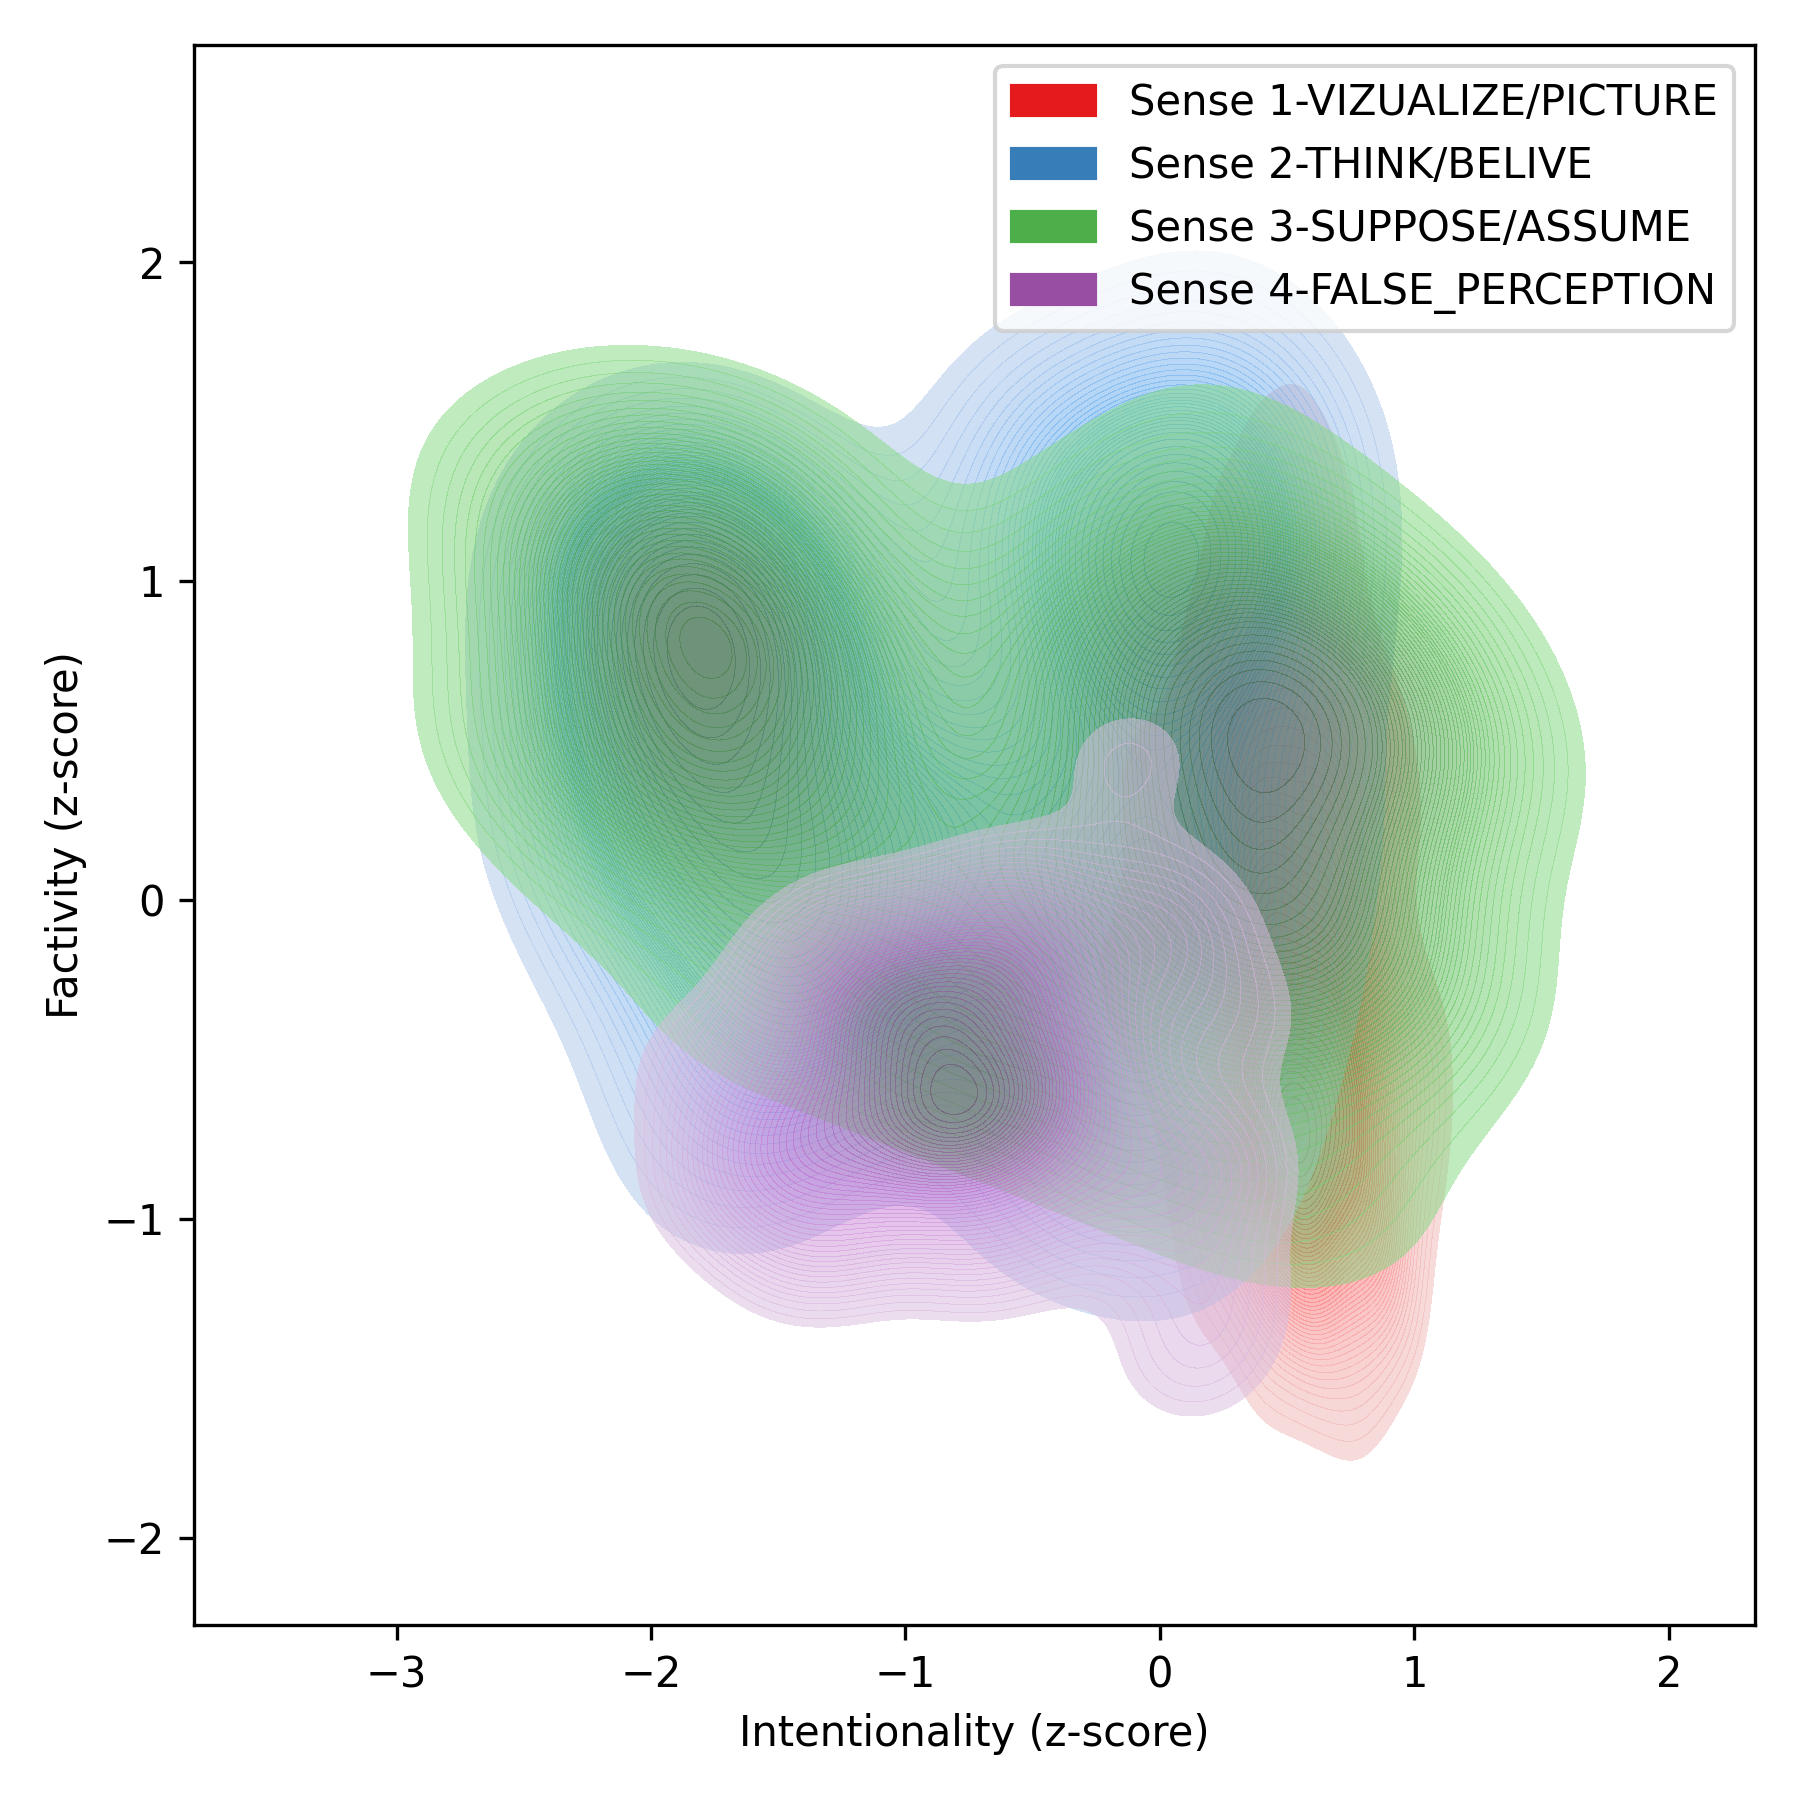
\includegraphics[width=\textwidth]{../../output/plots/embedding_projection_intentionality_factivity_2D_core_v3.png}
    \caption{Intentionality $vs$ factivity\label{fig:2D_IF}}
    \end{subfigure}
    \hfill
    \begin{subfigure}[b]{0.30\textwidth}
    \centering
    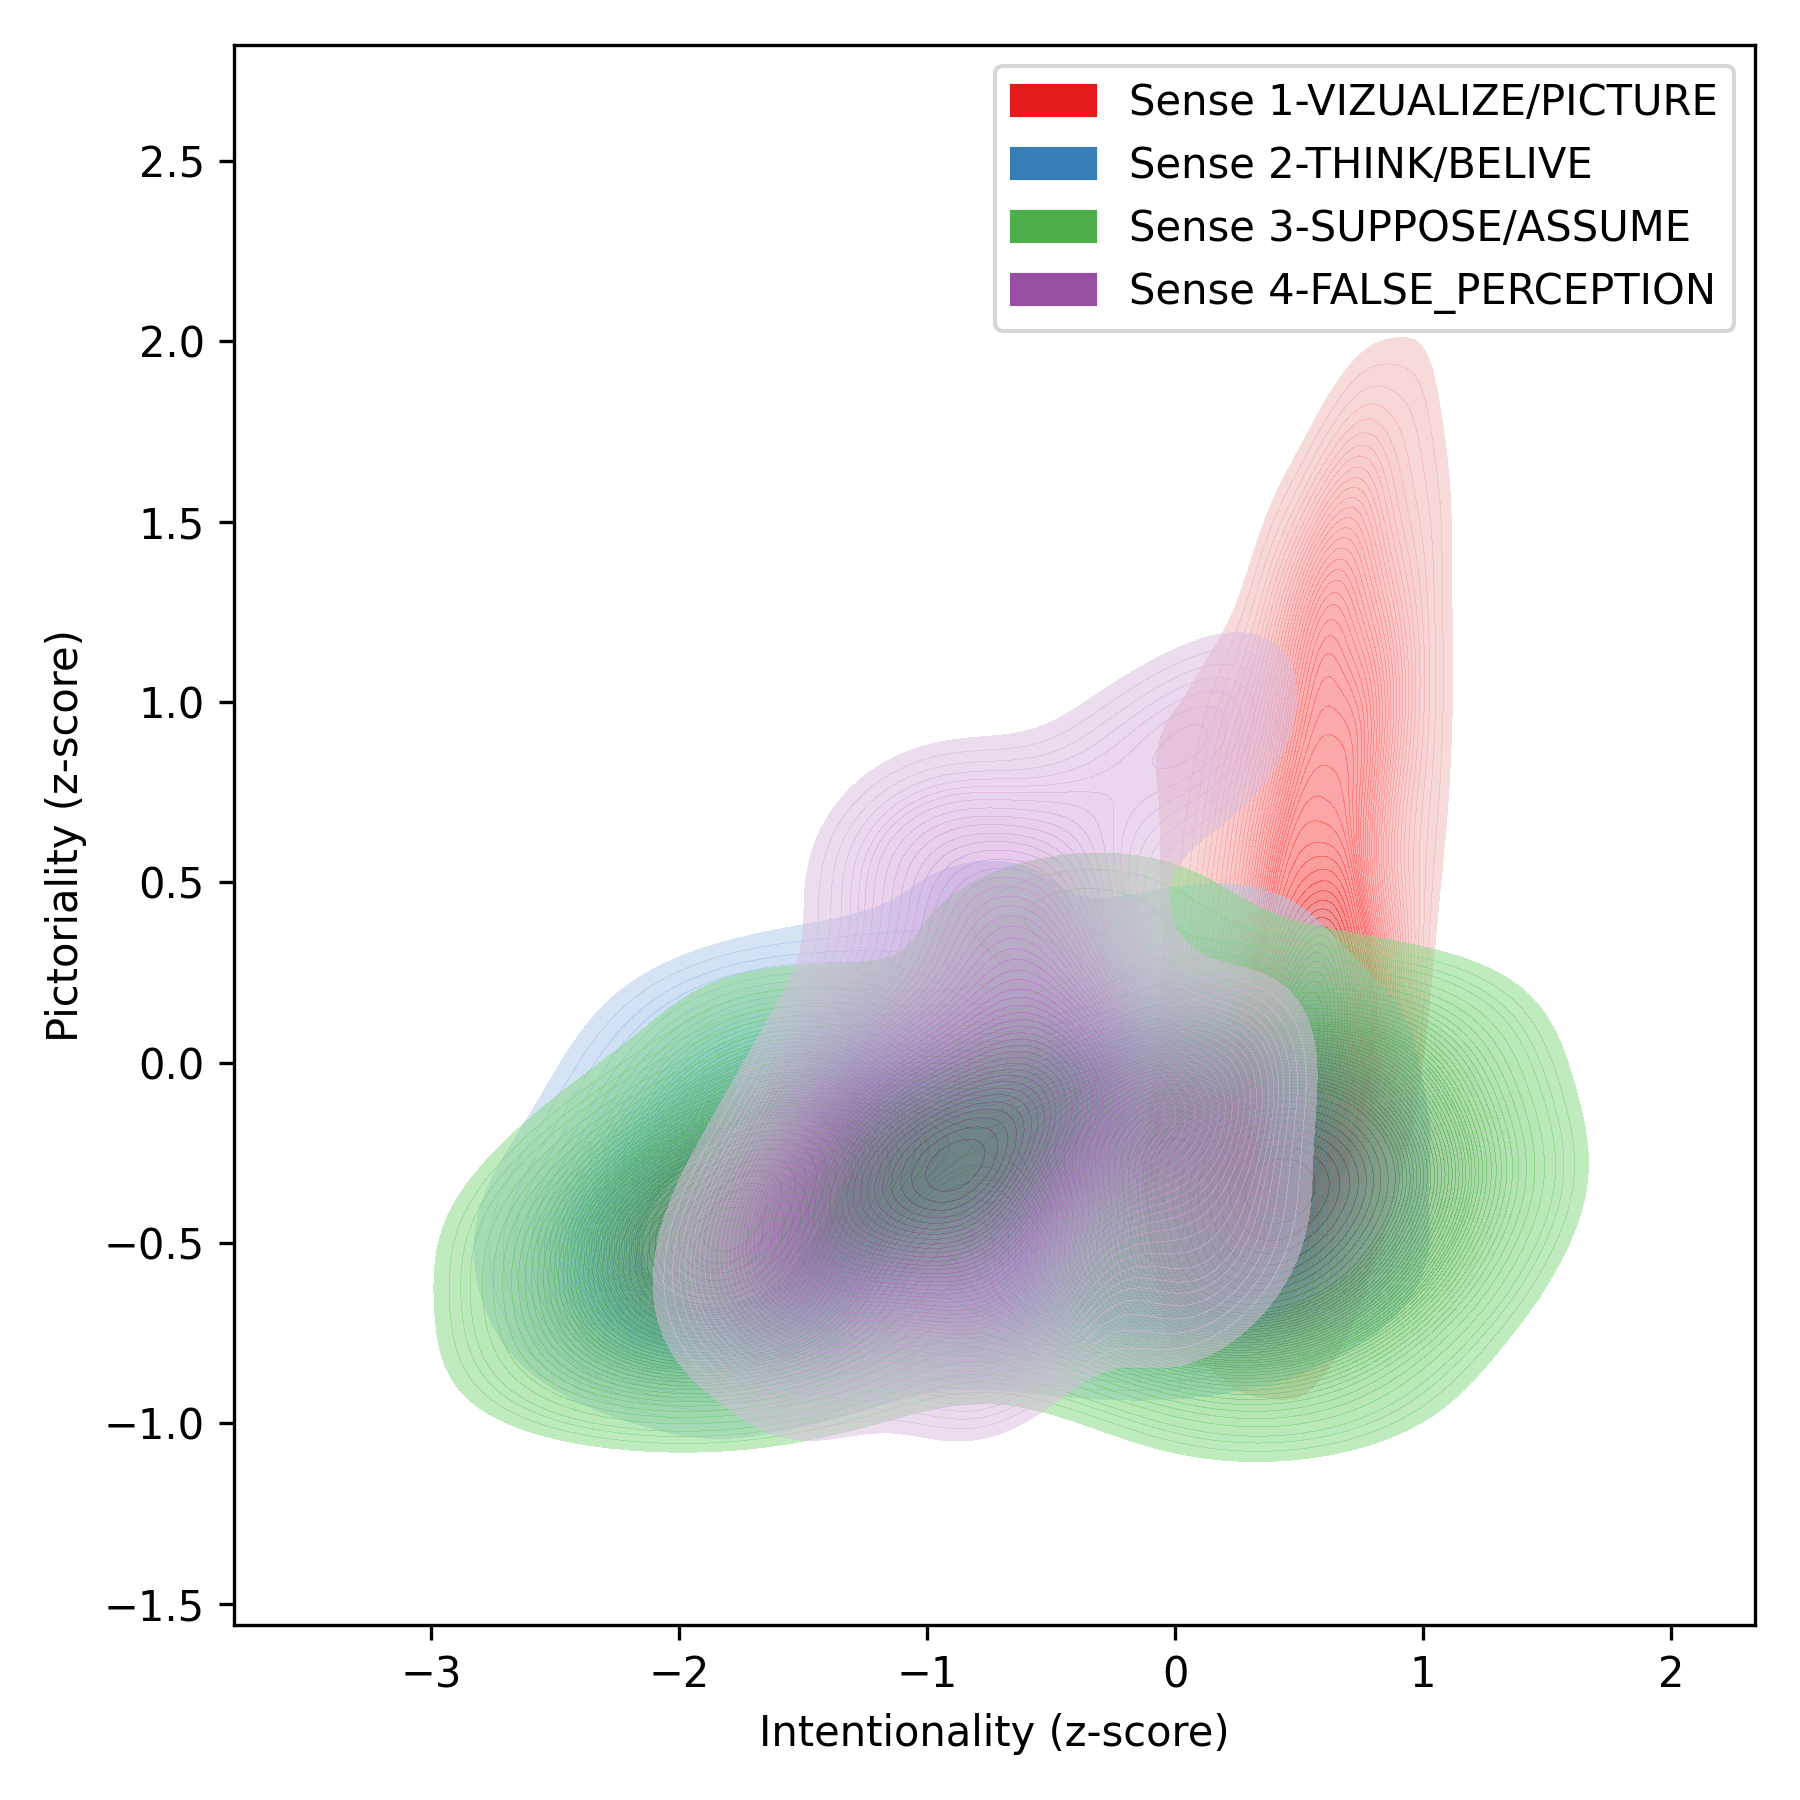
\includegraphics[width=\textwidth]{../../output/plots/embedding_projection_intentionality_pictoriality_2D_core_v3.png}
    \caption{Intentionality $vs$ pictoriality. \label{fig:2D_IP}}
    \end{subfigure}
    \hfill
    \begin{subfigure}[b]{0.30\textwidth}
    \centering
    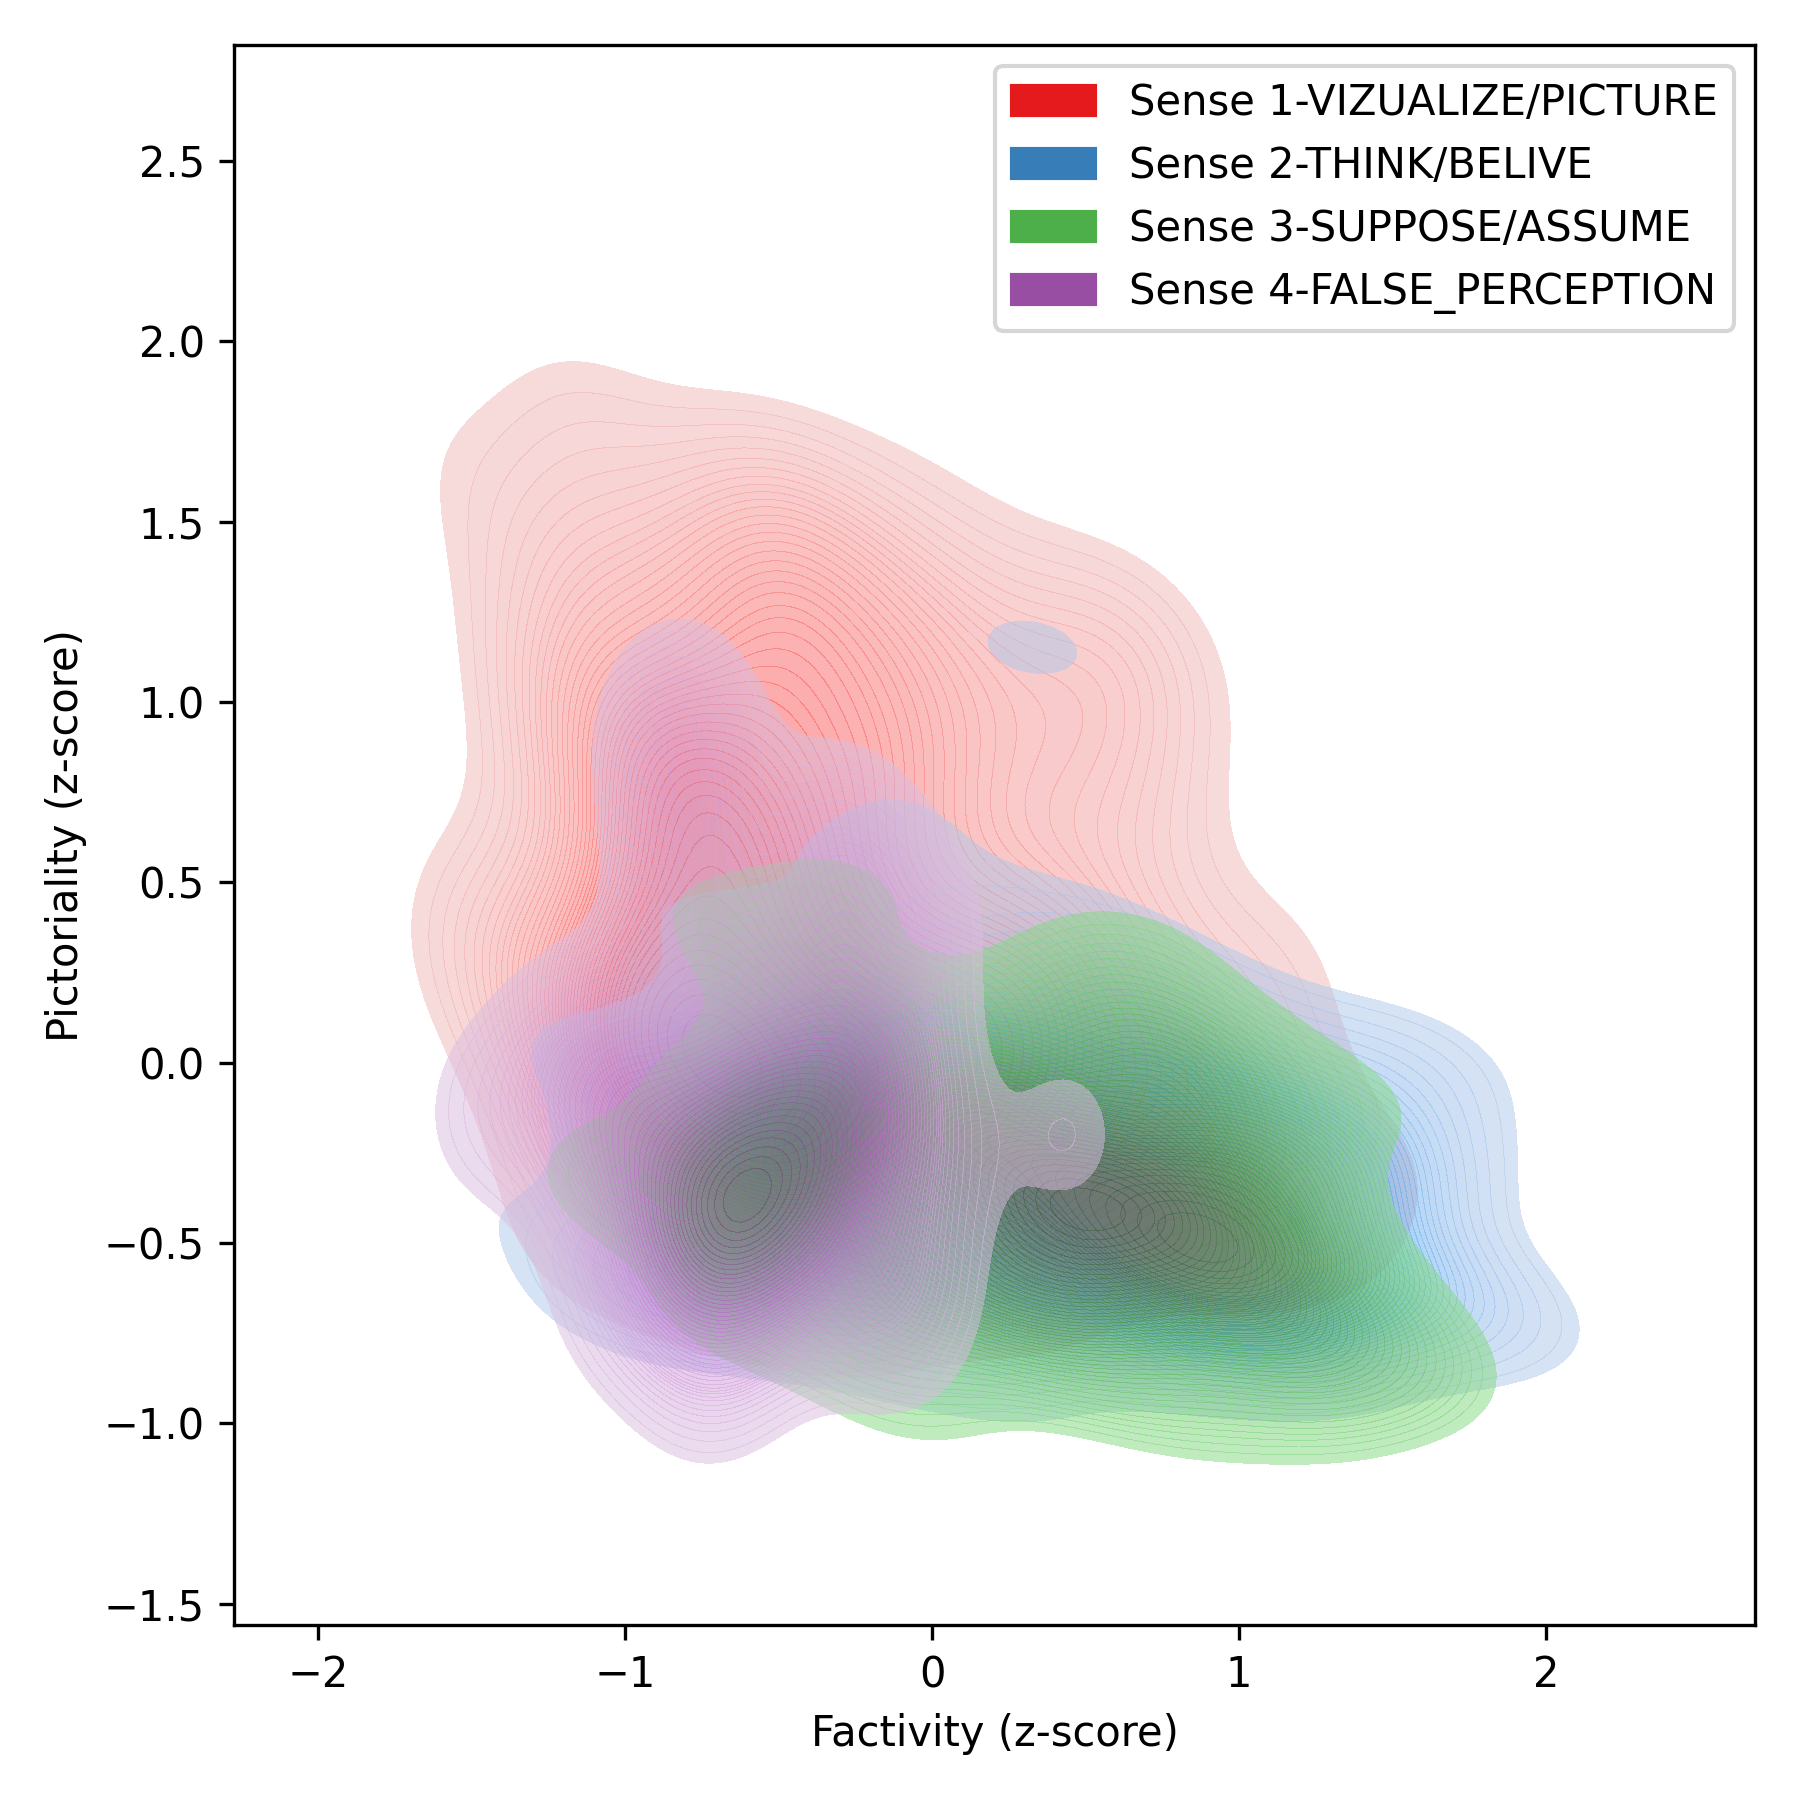
\includegraphics[width=\textwidth]{../../output/plots/embedding_projection_factivity_pictoriality_2D_core_v3.png}
    \caption{Factivity $vs$ pictoriality. \label{fig:2D_FP}}
    \end{subfigure}
\end{figure}

\subsection{Robustness check: sensitivity to embedding-layer
choice}\label{robustness-check-sensitivity-to-embedding-layer-choice}

Every analysis above uses the raw last hidden layer of BERT for each
token's embedding. The very last layer is somewhat specialized toward
BERT's masked-language-modeling pretraining objective, and
middle-to-late layers -- or an average across the last several layers --
have been reported elsewhere to sometimes carry semantic content at
least as well (e.g.~Ethayarajh 2019). We checked whether this choice
matters by repeating the centroid-based analysis with two alternatives:
the second-to-last hidden layer, and the average of the last four hidden
layers. The three variants were compared pairwise with two metrics
suited to what is actually being compared: Cohen's \(\kappa\) on each
token's nearest-centroid sense (a categorical assignment, for which
chance-corrected agreement is the natural fit), and Spearman's \(\rho\)
on the per-sense-pair centroid-overlap fractions from Figure
\ref{fig:centroidOverlapHeatmap} above (continuous scores, for which a
rank correlation between the score vectors shows directly whether the
variants agree on which sense pairs overlap most and least).

\begin{table}[H]
\centering
\caption{\label{tab:unnamed-chunk-28}Pairwise agreement between embedding-layer variants: nearest-centroid sense classification (Cohen's $\kappa$) and centroid-overlap fractions (Spearman $\rho$).\label{tab:variantAgreement}}
\centering
\begin{tabular}[t]{lrr}
\toprule
Variant pair & Cohen's $\kappa$ & Spearman $\rho$\\
\midrule
last vs avg last4 & 0.929 & 0.972\\
last vs second to last & 0.934 & 0.965\\
second to last vs avg last4 & 0.948 & 0.972\\
\bottomrule
\end{tabular}
\end{table}

Table \ref{tab:variantAgreement} shows that all three layer variants
agree closely: Cohen's \(\kappa\) ranges from 0.929 to 0.948
(conventionally interpreted as ``almost perfect'' agreement,
\(\kappa > 0.8\)), and Spearman's \(\rho\) ranges from 0.965 to 0.972.
In other words, which BERT layer(s) the token embedding is read from
does not materially change either which sense a token's embedding is
classified as (by nearest centroid) or the overall pattern of pairwise
sense overlap reported throughout this section. The last-layer
embeddings used above are therefore a reasonable, representative choice,
not an idiosyncratic one that happens to drive the reported conclusions.

\section{Appendix}\label{appendix}

\begin{landscape}\begin{table}[H]
\centering
\caption{\label{tab:unnamed-chunk-29}Pairwise KDE overlap coefficients between sense distributions for each feature. 
    $\hat{O}$ denotes the raw shared area under the minimum of two KDE curves; 
    $\hat{O}_{s1}$ and $\hat{O}_{s2}$ denote the fraction of sense 1 and sense 2's 
    distribution respectively that overlaps with the other, where values approaching 1 
    indicate near-complete distributional overlap.\label{tab:overlap}}
\centering
\fontsize{8}{10}\selectfont
\begin{tabular}[t]{lllrrr}
\toprule
Feature & Sense 1 ($S_1$) & Sense 2 ($S_2$) & $\hat{O}$ & $\hat{O}_{S_1}$ & $\hat{O}_{S_2}$\\
\midrule
intentionality & 1-VIZUALIZE/PICTURE & 1-VIZUALIZE/PICTURE & 0.212 & 0.214 & 0.226\\
intentionality & 1-VIZUALIZE/PICTURE & 1-VIZUALIZE/PICTURE & 0.307 & 0.309 & 0.343\\
intentionality & 1-VIZUALIZE/PICTURE & 1-VIZUALIZE/PICTURE & 0.220 & 0.222 & 0.231\\
intentionality & 2-THINK/BELIVE & 2-THINK/BELIVE & 0.675 & 0.742 & 0.820\\
intentionality & 2-THINK/BELIVE & 2-THINK/BELIVE & 0.762 & 0.838 & 0.830\\
intentionality & 3-SUPPOSE/ASSUME & 3-SUPPOSE/ASSUME & 0.655 & 0.796 & 0.714\\
factivity & 1-VIZUALIZE/PICTURE & 1-VIZUALIZE/PICTURE & 0.584 & 0.614 & 0.610\\
factivity & 1-VIZUALIZE/PICTURE & 1-VIZUALIZE/PICTURE & 0.608 & 0.633 & 0.631\\
factivity & 1-VIZUALIZE/PICTURE & 1-VIZUALIZE/PICTURE & 0.738 & 0.775 & 0.766\\
factivity & 2-THINK/BELIVE & 2-THINK/BELIVE & 0.936 & 0.960 & 0.972\\
factivity & 2-THINK/BELIVE & 2-THINK/BELIVE & 0.389 & 0.406 & 0.404\\
factivity & 3-SUPPOSE/ASSUME & 3-SUPPOSE/ASSUME & 0.409 & 0.424 & 0.422\\
pictoriality & 1-VIZUALIZE/PICTURE & 1-VIZUALIZE/PICTURE & 0.560 & 0.601 & 0.582\\
pictoriality & 1-VIZUALIZE/PICTURE & 1-VIZUALIZE/PICTURE & 0.483 & 0.519 & 0.523\\
pictoriality & 1-VIZUALIZE/PICTURE & 1-VIZUALIZE/PICTURE & 0.670 & 0.719 & 0.749\\
pictoriality & 2-THINK/BELIVE & 2-THINK/BELIVE & 0.771 & 0.808 & 0.834\\
pictoriality & 2-THINK/BELIVE & 2-THINK/BELIVE & 0.742 & 0.777 & 0.853\\
pictoriality & 3-SUPPOSE/ASSUME & 3-SUPPOSE/ASSUME & 0.662 & 0.717 & 0.761\\
\bottomrule
\end{tabular}
\end{table}
\end{landscape}

\begin{landscape}\begin{table}[H]
\centering
\caption{\label{tab:unnamed-chunk-30}Confusion Matrix.\label{tab:cm}}
\centering
\fontsize{8}{10}\selectfont
\begin{tabular}[t]{lrrrr}
\toprule
  & 1-VIZUALIZE/PICTURE & 2-THINK/BELIVE & 3-SUPPOSE/ASSUME & 4-FALSE\_PERCEPTION\\
\midrule
1-VIZUALIZE/PICTURE & 0.9710425 & 0.2544643 & 0.5434783 & 0.4067797\\
2-THINK/BELIVE & 0.0289575 & 0.7366071 & 0.4347826 & 0.4745763\\
3-SUPPOSE/ASSUME & 0.0000000 & 0.0000000 & 0.0000000 & 0.0000000\\
4-FALSE\_PERCEPTION & 0.0000000 & 0.0089286 & 0.0217391 & 0.1186441\\
\bottomrule
\end{tabular}
\end{table}
\end{landscape}

  \bibliography{hb.bib}

\end{document}
